\chapter{Cross section calculation}

\section{Kinematical variables}
\label{kin_var}

After the double-pion event selection that uses the missing mass technique, the four-momenta of all particles are known and can be used for  the calculation of all  kinematic variables. The cross sections are obtained in the single-photon exchange approximation in the center of mass frame of the {\em virtual photon -- initial proton} system.

\begin{figure}[htp]
\begin{center}
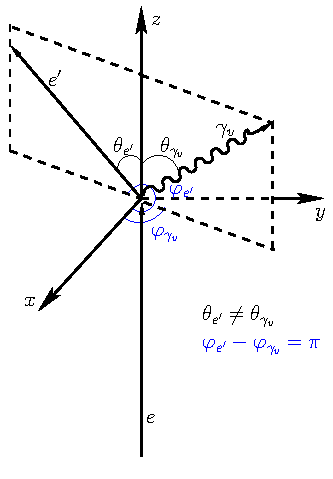
\includegraphics[width=6cm]{pictures/cross_sction/luminosity/electron_angles.pdf}
\caption{\small Virtual photon and scattered electron angles $\theta$ and $\varphi$ in the lab frame.} \label{fig:cr_sec_el_angles}
\end{center}
\end{figure}

Therefore, to calculate the kinematic variables the four-momenta of all particles need to be transformed from the lab frame to the c.m. frame.  For that purpose Lorentz transformations that include the following steps are used~\footnote[1]{In all derivations the energy is assumed to be the last component of the four-momentum and the four-momentum to be a row vector.}.

1) Firstly $(xy)$-plane of the lab system is rotated around $z$-axis to make $x$-axis laying in the electron scattering plane (see Fig.~\ref{fig:cr_sec_el_angles}). This rotation transforms the  four-momentum as $P' = P*R_1$, 
with 
\begin{equation}
R_{1} = \begin{pmatrix}
 cos(\varphi_{e'})& -sin(\varphi_{e'}) & 0 &0 \\ 
 sin(\varphi_{e'})& cos(\varphi_{e'}) &  0& 0\\ 
0 & 0 & 1 &0 \\ 
 0&  0&  0&1 
\end{pmatrix},
\end{equation}
where $\varphi_{e'}$ is the azimuthal angle of the scattered electron.

After this rotation $\varphi_{\gamma_v} = \pi$, since the $\varphi$ angle between scattered electron and virtual photon is equal to $\pi$; and after the rotation $\varphi_{e'} = 0$ with respect to the intermediate reference frame.

2) After that the lab system is rotated to align the $z$-axis with the virtual photon direction. The four-momentum transformation for this rotation is given by $P'' = P'*R_2$, with 
\begin{equation}
R_{2}=\begin{pmatrix}
cos(\theta_{\gamma_{v}}) &0  &-sin(\theta_{\gamma_{v}})  &0 \\ 
 0& 1 & 0 &0 \\ 
 sin(\theta_{\gamma_{v}}) &0  &cos(\theta_{\gamma_{v}})  & 0\\ 
0 &0  & 0 &1 
\end{pmatrix},
\end{equation}
where $\theta_{\gamma_v}$ is the polar angle of the virtual photon.~\footnote[2]{Using embedded ROOT functions, both rotations can be coded using the unit vectors TVector3~$uz$~=~P4\_gamma.Vect().Unit() and 
 TVector3~$ux$~=~(P4\_EL.Vect().Cross(P4\_ELP.Vect())).Unit(), where P4\_gamma, P4\_EL, and P4\_ELP are the four-momenta of the virtual photon, initial and final electrons, respectively. 
 The axis vector $ux$ needs to be rotated according to $ux$.Rotate(3.*M\_PI/2,$uz$).
Finally the rotation is defined as rot.SetZAxis($uz$,$ux$).Invert() and needs to be applied to the four-momentum (P4) of each particle:
 P4.Transform(rot).}

3) Finally a boost into the c.m. frame of the {\em virtual photon -- initial proton} system is performed. It is given by the formula $P''' = P''*R_3$, with 
\begin{equation}
R_{3} = \begin{pmatrix}
1 &0  &0  &0 \\ 
0 &1  &0  &0 \\ 
 0&  0& \gamma  &-\gamma \beta  \\ 
 0&  0& -\gamma \beta  & \gamma 
\end{pmatrix}, \, \, \, \beta =\frac{|\overrightarrow{q}|}{E_{\gamma }+m_{proton}}=\frac{\sqrt{E^{2}_{\gamma }+Q^{2}}}{E_{\gamma }+m_{proton}}, \, \, \,\,  \gamma =\frac{1}{\sqrt{1-\beta ^{2}}},
\end{equation}
where $|\overrightarrow{q}|$ is the magnitude of the three-vector of the virtual photon and $\beta$ the magnitude and $z$-component of the three-vector $\overrightarrow{\beta}=(0,0,\beta)$.~\footnote[3]{
Note: if you use ROOT function .Boost you should change the sign of the $z$-component of $\beta$-vector: .Boost(0,0,-$\beta$).}


When the four-momenta of all particles in the c.m. frame are defined one can calculate the kinematic variables that describe the final hadron state.
The three-body final state is 
unambiguously determined by five kinematic
variables. Indeed, three final particles could be
described by $4 \times 3 = 12$ components of
their four-momenta. All these particles are
on mass shell. So, it gives us three restrictions
$E_{i}^{2} -P_{i}^{2} =
m_{i}^{2}$~$(i=1,2,3)$. The energy-momentum
conservation imposes four additional constraints
for the final particles four-momenta
components. So, eventually five
kinematic variables remain, which determine
unambiguously the three-body final state
kinematics. In the electron scattering process $e
p \rightarrow e' p' \pi^{+} \pi^{-}$ 
the variables $W$, $Q^{2}$ are also present besides
the hadronic final state variables. So
electron scattering cross section for double-charged pion electroproduction should be
seven-differential: five variables for the final
hadrons plus $W$ and $Q^{2}$ that are determined by the
scattered electron kinematics. Such
seven-differential cross sections may be
written as
$\frac{d^{7}\sigma}{dWdQ^{2}d^{5}\tau}$,
where $d^{5}\tau$ is five-dimensional phase space differential.

Several sets of five variables for
the description of the final hadron kinematics may
be used. The following generalized set of
variables is used in this analysis:
\begin{itemize}
\item invariant mass of the first pair of the
particles $M_{12}$;
\item invariant mass of the second pair of the
particles $M_{23}$;
\item the first particle solid angle $\Omega$;
\item the angle between two planes: one of
them (plane A) is defined by the three-momenta of
the virtual photon (or initial proton) and the first final hadron, the second
plane (plane B) is defined by the three-momenta of all final hadrons (these angles are shown in  Figs.~\ref{fig:cr_sec_kinematic1},~\ref{fig:cr_sec_kinematic2},~\ref{fig:cr_sec_kinematic3} for various choices of the first particle).
\end{itemize}

The cross sections in this analysis are obtained in three sets of variables depending on
various assignments for the first, second, and
third final hadrons:
\begin{itemize}
\item invariant mass of the $p'\pi^{+}$ pair, invariant mass of the $\pi^{+}\pi^{-}$
pair, proton spherical angles $\theta_{p'}$ and $\varphi_{p'}$ and 
angle $\alpha_{(p,p')(\pi^{+},\pi^{-})}$ (or $\alpha_{p'}$) 
between planes B (defined by the momenta of
all final hadrons) and A  (defined by
initial and final protons), see Fig.~\ref{fig:cr_sec_kinematic1};
% of the pion pair with respect to the plane composed by initial
%and final protons;
\item invariant mass of the $\pi^{-}\pi^{+}$
pair, invariant mass of the $\pi^{+}p$
pair, $\pi^{-}$ spherical angles
$\theta_{\pi^{-}}$ and $\varphi_{\pi^{-}}$
and angle 
$\alpha_{(p\pi^{-})(p'\pi^{+})}$ (or $\alpha_{\pi^{-}}$)
between planes B (defined by the momenta of
all final hadrons) and A  (defined by
initial proton and $\pi^{-}$), see Fig.~\ref{fig:cr_sec_kinematic2};
%of the $p\pi^{+}$ pair with respect to the plane composed by
%initial proton and $\pi^{-}$;
\item invariant mass of the $\pi^{+}\pi^{-}$
pair, invariant mass of the $\pi^{-}p$
pair, $\pi^{+}$ spherical angles
$\theta_{\pi^{+}}$ and $\varphi_{\pi^{+}}$
and angle
$\alpha_{(p\pi^{+})(p'\pi^{-})}$ (or $\alpha_{\pi^{+}}$)
between planes B (defined by the momenta of
all final hadrons) and A  (defined by
initial proton and $\pi^{+}$), see Fig.~\ref{fig:cr_sec_kinematic3}.
%of the $p\pi^{-}$ pair with respect to the plane composed by initial 
%proton and $\pi^{+}$.
\end{itemize}

%It needs to be mentioned that in c.m. frame total three-momentum of the initial particles is equal to zero, so three-momenta of all final hadrons should compensate eache other and they are necesserily laying in one plane.

Lets explain in more detail the calculation of the kinematical variables in case of set number two.  The invariant masses $
M_{\pi^{+}\pi^{-}}$ and $M_{\pi^{+}p'}$
  are calculated from the four-momenta of the final 
particles $P_{\pi^{-}}$, $P_{\pi^{+}}$, $P_{p'}$ in the c.m. frame in the following way
\begin{equation}
\begin{aligned}
M_{\pi^{+}\pi^{-}} = \sqrt{(P_{\pi^{+}} + P_{\pi^{-}})^{2}} & \text{  and}\\ \label{invmasses}
M_{\pi^{+}p'} = \sqrt{(P_{\pi^{+}} + P_{p'})^{2}}. & \\ 
\end{aligned}  
\end{equation}  

The angle $\theta_{\pi^{-}}$ between the three-momentum of the initial photon ($\vec P_{\gamma}$) and three-momentum of the final $\pi^{-}$ ($\vec P_{\pi^{-}}$) in 
c.m. frame is calculated as:
\begin{equation}
\theta_{\pi^{-}} = acos\left( \frac{(\vec P_{\pi^{-}} \cdot \vec P_{\gamma})}
{|\vec P_{\pi^{-}}| |\vec P_{\gamma}|} \right)
\label{angletheta}
\end{equation} 


The angle $\varphi_{\pi^{-}}$ is determined as:
\begin{equation}
\begin{aligned}
\varphi_{\pi^{-}} = arctg\left( \frac{P_{y
\pi^{-}}}{P_{x\pi^{-}}} \right)\!; & \text{ }
P_{x\pi^{-}} > 0 ; P_{y\pi^{-}} > 0 \\
\varphi_{\pi^{-}} = arctg\left( \frac{P_{y
\pi^{-}}}{P_{x\pi^{-}}} \right) + 2\pi; & \text{ }
P_{x\pi^{-}} > 0 ; P_{y\pi^{-}} < 0 \\
\varphi_{\pi^{-}} = arctg\left( \frac{P_{y
\pi^{-}}}{P_{x\pi^{-}}} \right) + \pi; & \text{ }
P_{x\pi^{-}} < 0 ; P_{y\pi^{-}} < 0 \\
\varphi_{\pi^{-}} = arctg\left( \frac{P_{y
\pi^{-}}}{P_{x\pi^{-}}} \right) + \pi; & \text{ }
P_{x\pi^{-}} < 0 ; P_{y\pi^{-}} > 0  \\
\varphi_{\pi^{-}} = \pi/2; & \text{ }
P_{x\pi^{-}} = 0 ; P_{y\pi^{-}} > 0  \\
\varphi_{\pi^{-}} = 3\pi/2; & \text{ }
P_{x\pi^{-}} = 0 ; P_{y\pi^{-}} < 0, 
\end{aligned}
\end{equation}
where $P_{i\pi^{-}}$ is $i$-component of the $\pi^{-}$ three-momentum ($i = x,y,z$).
The angles $\theta_{\pi^{-}}$ and $\varphi_{\pi^{-}}$ are shown in Fig.~\ref{fig:cr_sec_thetaphi}.

The calculation of the angle $\alpha_{\pi^{-}}$
 between two planes A and B (see Fig.~\ref{fig:cr_sec_kinematic2})
is more complicated. Firstly two
auxiliary vectors $\vec \gamma$  and
$\vec \beta$ should be determined. The vector $\vec \gamma$ is the unit vector perpendicular to the three-momentum
$\vec P_{\pi^{-}}$, directed toward the vector $(-\vec n_{z})$ and situated in the plane A, which is defined by 
the three-momentum of initial proton and three-momentum of $\pi^{-}$. $\vec
n_{z}$ is the unit vector directed along $z$-axis.
The vector $\vec \beta$ is the unit vector perpendicular to the three-momentum of $\pi^{-}$, 
directed toward the three-momentum of $\pi^{+}$ and situated in the plane B, which is defined 
by all final hadrons. Note that the three-momenta of $\pi^{+}$,
$\pi^{-}$, $p'$ are in the same plane, since in c.m. frame
their total three-momentum has to be equal to zero.
 Then the angle between two planes  $\alpha_{\pi^{-}}$ is
\begin{equation}
\alpha_{\pi^{-}} = acos(\vec \gamma \cdot \vec \beta),
\label{eq:cr_sec_anglealpha}
\end{equation}
where $acos$ is a function that runs between zero and
$\pi$, while the angle $\alpha_{\pi^{-}}$ may vary between zero and
$2\pi$. To determine the $\alpha$ angle in the
range between $\pi$ and $2\pi$ 
the relative direction between the $\pi^{-}$ three-momentum and the vector product $\vec \delta = [ \vec \gamma \times \vec \beta ]$ of the auxiliary vectors $\vec
\gamma$ and $\vec \beta$ should be taken into account.
%\begin{equation}
%\vec \delta = [ \vec \gamma \times \vec \beta ]
%\label{vecprod}
%\end{equation}
If the vector $\vec \delta$ is colinear to the three-momentum of $\pi^{-}$, the angle $\alpha_{\pi^{-}}$ is determined
by~(\ref{eq:cr_sec_anglealpha}), and in a case of anti-collinearity by
\begin{equation}
\alpha_{\pi^{-}} = 2\pi - acos(\vec \gamma \cdot \vec \beta).
\label{eq:cr_sec_anglealpha_var}
\end{equation}
The defined above vector $\vec \gamma$ can be expressed as
\begin{eqnarray}
\vec \gamma = a_{\alpha}(-\vec n_{z}) + b_{\alpha}\vec n_{P_{\pi^{-}}} & \text{with} \nonumber \\
a_{\alpha} = \sqrt{\frac{1}{1 - (\vec n_{P_{\pi^{-}}} \cdot (-\vec n_{z} ) )^{2}}} & \text{and} \label{alphavec}\\
b_{\alpha} = - (\vec n_{P_{\pi^{-}}} \cdot (-\vec n_{z} ) ) a_{\alpha} \textrm{ ,} \nonumber
\end{eqnarray} 
where $\vec n_{P_{\pi^{-}}}$ is the unit vector directed along the three-momentum of $\pi^{-}$ (see Fig.~\ref{fig:cr_sec_kinematic2}).

Taking the scalar products $(\vec \gamma \cdot \vec
n_{P_{\pi^{-}}})$ and $(\vec \gamma \cdot \vec  \gamma)$,
it is straightforward to verify, that $\vec \gamma$ is the unit vector perpendicular to the three-momentum of $\pi^{-}$.

The vector $\vec \beta$ can be obtained as
\begin{eqnarray}
\vec \beta = a_{\beta}\vec n_{P_{\pi^{+}}} + b_{\beta}\vec n_{P_{\pi^{-}}} & \text{with} \nonumber \\
a_{\beta} = \sqrt{\frac{1}{1 - (\vec n_{P_{\pi^{+}}} \cdot \vec n_{P_{\pi^{-}}})^{2}}} & \text{and} \label{betavec}\\
b_{\beta} = - (\vec n_{P_{\pi^{+}}} \cdot \vec n_{P_{\pi^{-}}}) a_{\beta} \textrm{ ,} \nonumber
\end{eqnarray} 
where $\vec n_{P_{\pi^{+}}}$ is the unit vector directed along the three-momentum of $\pi^{+}$.

Again taking the scalar products $(\vec \beta \cdot \vec
n_{P_{\pi^{-}}})$ and $(\vec \beta \cdot \vec  \beta)$,
it is straightforward to see, that $\vec \beta$ is
the unit vector perpendicular to the 
three-momentum of $\pi^{-}$. 

The angle $\alpha_{\pi^{-}}$ coincides with
 the angle between the vectors $\vec \gamma$ and
$\vec \beta$.
So, the scalar product $( \vec \gamma \cdot
\vec \beta )$ allows to determine the angle
$\alpha_{\pi^{-}}$~(\ref{eq:cr_sec_anglealpha}). The kinematic
variables for  the other assignments for the
first, second, and third final hadrons
described above, are evaluated in the similar
way.
\begin{figure}[htp]
\begin{center}
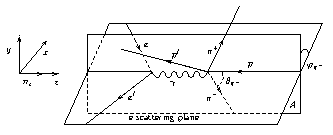
\includegraphics[width=12cm]{pictures/cross_sction/angles/thetaphi.pdf}
\caption{\small Polar ($\theta_{\pi^{-}}$) and azimutal ($\varphi_{\pi^{-}}$) angles of $\pi^{-}$ in the c.m. frame.} \label{fig:cr_sec_thetaphi}
\end{center}
\end{figure}
\begin{figure}[htp]
\begin{center}
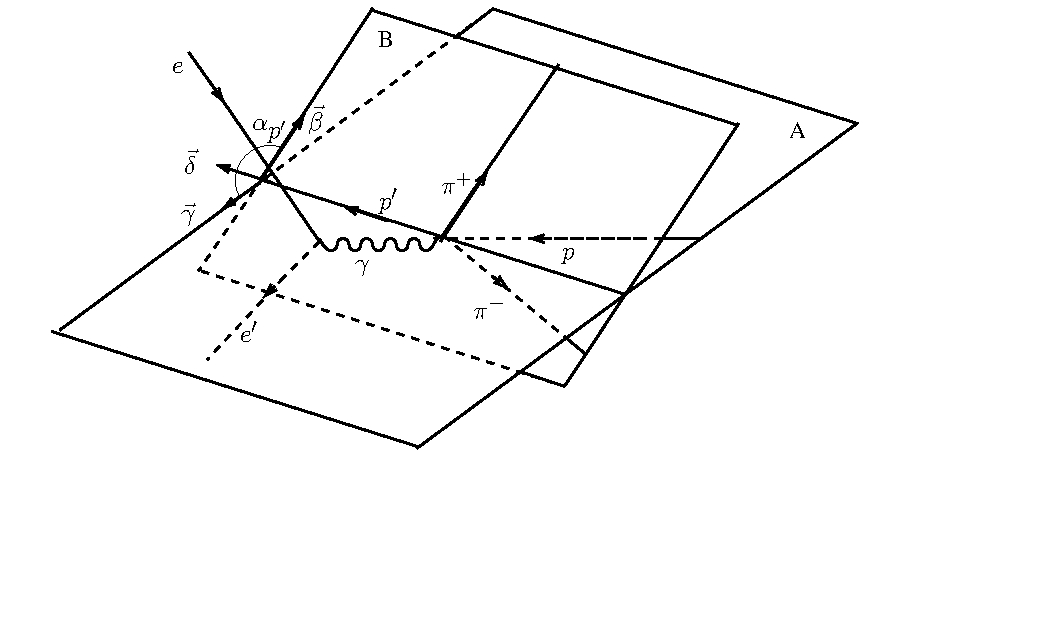
\includegraphics[width=12cm]{pictures/cross_sction/angles/alpha2.pdf}
\caption{\small Definition of the angle $\alpha_{p'}$ between two planes: the plane B is defined by the three-momenta of all final hadrons, while the plane A defined by  the three-momenta of initial and scattered protons. The definitions of  auxiliary vectors $\vec \beta$, $\vec \gamma$, $\vec \delta$ are given in the text.} \label{fig:cr_sec_kinematic1}
\end{center}
\end{figure}

\begin{figure}[htp]
\begin{center}
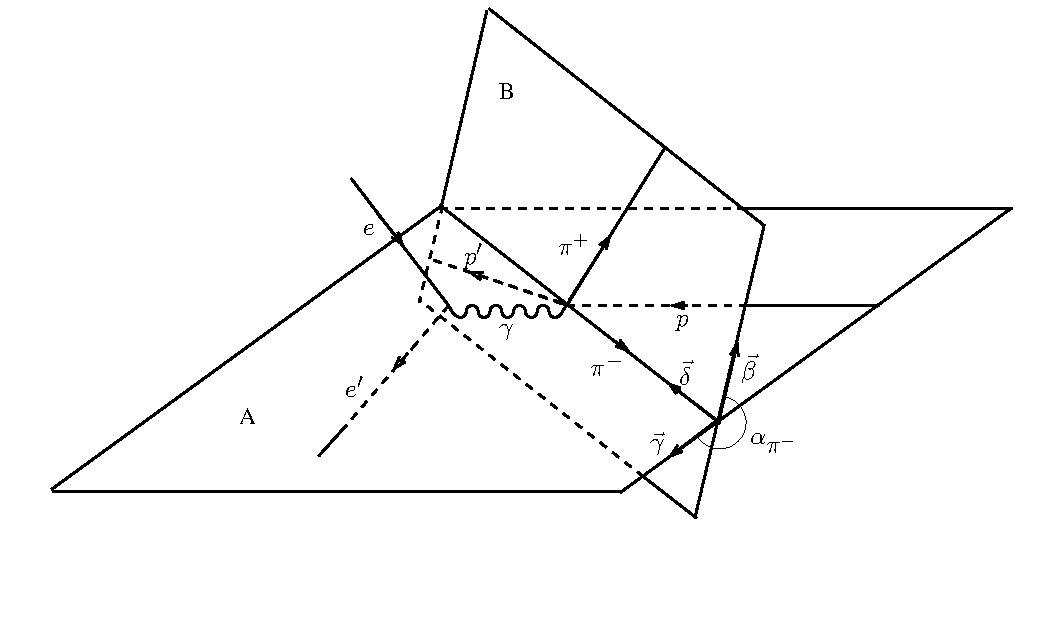
\includegraphics[width=12cm]{pictures/cross_sction/angles/alpha1.pdf}
\caption{\small Definition of the angle $\alpha_{\pi^{-}}$ between two planes: the plane B is defined by the three-momenta of all final hadrons, while the plane A defined by  the three-momenta of $\pi^{-}$ and scattered proton. The definitions of  auxiliary vectors $\vec \beta$, $\vec \gamma$, $\vec \delta$ are given in the text.} \label{fig:cr_sec_kinematic2}
\end{center}
\end{figure}



\begin{figure}[htp]
\begin{center}
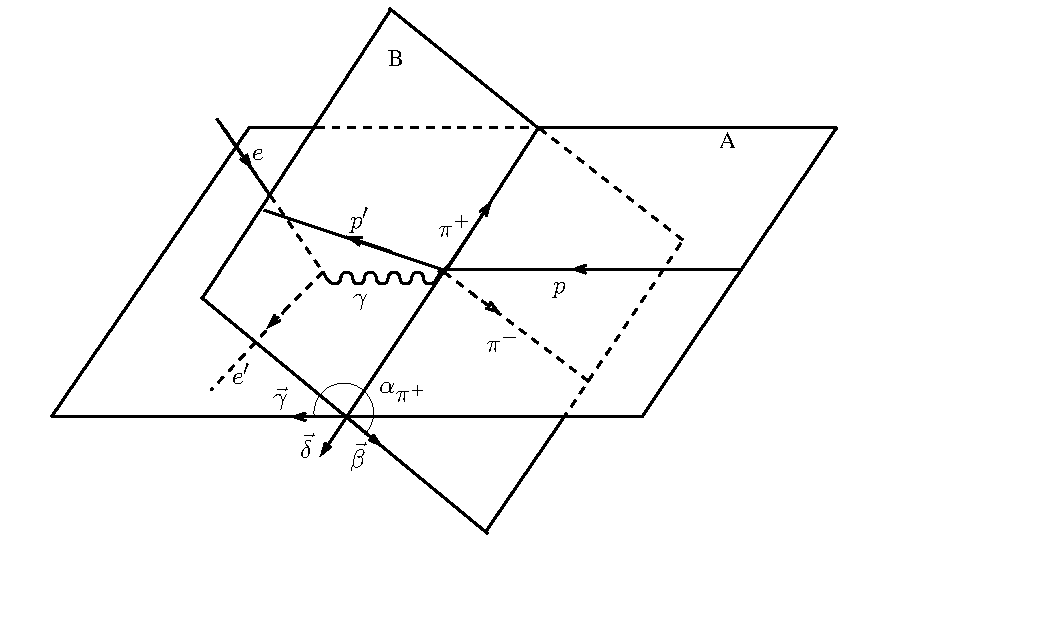
\includegraphics[width=12cm]{pictures/cross_sction/angles/alpha3.pdf}
\caption{\small Definition of the angle $\alpha_{\pi^{+}}$ between two planes: the plane B is defined by the three-momenta of all final hadrons, while the plane A defined by  the three-momenta of $\pi^{+}$ and scattered proton. The definitions of  auxiliary vectors $\vec \beta$, $\vec \gamma$, $\vec \delta$ are given in the text.} \label{fig:cr_sec_kinematic3}
\end{center}
\end{figure}

Further detailed information about kinematic of the reactions with three-particle final states can be found here~\cite{Byckling:1971vca}.


\section{Cross section formula}
\label{cr_sec_formula}

\begin{figure}[htp]
\begin{center}
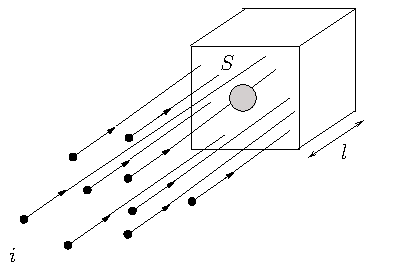
\includegraphics[width=6cm]{pictures/cross_sction/luminosity/luminosity_new.pdf}
\caption{\small The incoming electron beam with the current $i$ is hitting a homogeneous target with the area $S$ and density $\rho$.} \label{fig:cr_sec_Luminosity}
\end{center}
\end{figure}

In the fixed target experiments (see Fig.~\ref{fig:cr_sec_Luminosity}) the interaction rate (the number of interactions per second) can be determined according to the following relation:

\begin{equation}
\frac{dN}{dt}=\frac{iN_{targ}\sigma}{S},
\label{eq:cr_sec_rate}
\end{equation} 
where $i$ is the beam current (the number of incoming electrons per second), $N_{targ}$ is the total number of nuclei inside the target, $S$ is the taget area, $\sigma$ is the total cross section.

For $i$ the following is true:

\begin{equation}
i=\frac{dN_{beam}}{dt}=\frac{1}{q_{e}}\frac{dQ}{dt},
\label{eq:cr_sec_j}
\end{equation} 
where $N_{beam}$ is the number of incoming electrons, $Q$ is the total charge that is carried by incoming electrons, $q_{e}$ is the elementary charge.

$N_{targ}$ can be written in this way:

\begin{equation}
N_{targ}=\frac{mN_{A}}{M_{m}}=\frac{N_{A}\rho V}{M_{m}}=\frac{N_{A}\rho Sl}{M_{m}},
\label{eq:cr_sec_n_targ}
\end{equation} 
where $m$, $V$, $\rho$, $l$ are the mass, volume, density and length of the target, respectively, $M_{m}$ is the molar mass of the target material, $N_{A}$ is the Avogadro constant.


From (\ref{eq:cr_sec_rate}), (\ref{eq:cr_sec_j}) and (\ref{eq:cr_sec_n_targ}) the cross section
\begin{equation}
\sigma =\frac{q_{e}\Delta NM_{m}}{QlN_{A}\rho }=\frac{\Delta N}{L},
\label{eq:cr_sec_total_cr_sec}
\end{equation}  
where $L=\frac{QlN_{A}\rho }{q_{e}M_{m}}$ is the luminosity and $Q$ is the total charge of incoming electrons accumulated in the Faraday cup.

Since this analysis is focused on the reaction $e p \rightarrow e' p' \pi^{+} \pi^{-}$, the quantity  $\Delta N$ in the formula (\ref{eq:cr_sec_total_cr_sec}) is the total number of double-pion events. Liquid hydrogen is located in the target cell, hence the number of events that correspond to the target cell walls needs to be subtracted from the number of events that corresponds to the full target. 

Taking into account that the charge accumulated in the Faraday cup is different for full ($Q_{full}$) and empty ($Q_{empty}$) target runs the formula for the total  cross section can be rewritten as
\begin{equation}
\sigma =\frac{\frac{\Delta N_{full}}{Q_{full}}- \frac{\Delta N_{empty}}{Q_{empty}}}{\frac{l\rho N_{A}}{q_{e}M_{m}}}.
\label{eq:cr_sec_total_cr_sec2}
\end{equation}  

As it is mentioned in Sect.~\ref{kin_var} the double-pion cross section depends on seven kinematical variables. 
For the second set of kinematical
variables (see Sect.~\ref{kin_var}) considering formula (\ref{eq:cr_sec_total_cr_sec2}) the seven-differential cross section can be
written as 
\begin{equation}
\frac{d\sigma}{dWdQ^{2}dM_{p\pi^{+}}dM_{\pi^{+}\pi^{-}}d\Omega
d\alpha_{\pi^{-}}} = \frac{1}{F \cdot R} 
\frac{\left( \frac{\Delta N_{full}}{Q_{full}}-\frac{\Delta N_{empty}}{Q_{empty}} \right)}{
\Delta W \Delta Q^{2} \Delta \tau \left( \frac{l \rho N_{A}}{q_{e}M_{H}} \right)} \textrm{ ,}
\label{expcrossect}
\end{equation}
where $\Delta N_{full}$ and $\Delta N_{empty}$ are the numbers of events inside the
seven-dimensional bin for runs with hydrogen and
empty target, respectively, $F$ is total efficiency
 coming from the  Monte Carlo simulation,
$R$ is the
radiative correction factor,  $Q_{full}$ and $Q_{empty}$ are the integrated Faraday cup charges for runs with hydrogen and empty target, respectively, $q_{e}$ is the elementary charge ($q_{e} =1.610^{-19} $C), $\rho$ is the density of liquid hydrogen ($\rho = 0.0708 $ g/cm$^{3}$) at $T = 20$~K,
$l$ is the length of the target ($l = 2$ cm), $M_{H}$ is the molar density of
the natural mixture of hydrogen ($M_{H} = 1.00794$ g/mol),  $N_{A}$ is Avogadro's
number ($N_{A} =6.0210^{23}$ mol$^{-1}$),  $\Delta
W$ and $ \Delta Q^{2}$ are kinematical bins that are determined by the electron
scattering
 kinematics, and $\Delta \tau$ is an element of the
 hadronic five-dimensional phase space

\begin{equation}
\Delta \tau = \Delta M_{p\pi^{+}} \Delta
M_{\pi^{+}\pi^{-}} \Delta
(-cos(\theta_{\pi^{-}})) \Delta
\varphi_{\pi^{-}} \Delta \alpha_{\pi^{-}}.
\label{multibin}
\end{equation}


In the single photon exchange approximation,
the electron scattering cross section is related
to the hadronic cross section $\frac{d\sigma}{dM_{p\pi^{+}}dM_{\pi^{+}\pi^{-}}d\Omega_{\pi^{-}}
d\alpha_{\pi^{-}}}$ by

\begin{equation}
\frac{d\sigma}{dM_{p\pi^{+}}dM_{\pi^{+}\pi^{-}}d\Omega_{\pi^{-}}
d\alpha_{\pi^{-}}} = \frac{1}{\Gamma_{v}}
\frac{d\sigma}{dWdQ^{2}dM_{p\pi^{+}}dM_{\pi^{+}\pi^{-}}d\Omega_{\pi^{-}}
d\alpha_{\pi^{-}}}  \textrm{ ,}
\label{fulldiff}
\end{equation}
where $\Gamma_{v}$ is 
virtual photon flux, given by

\begin{equation}
\Gamma_{v} =
\frac{\alpha}{4\pi}\frac{1}{E_{beam}^{2}M_{p}^{2}}\frac{W(W^{2}-M_{p}^{2})}
{(1-\varepsilon)Q^{2}} \textrm{ ,}
\label{flux}
\end{equation}
where $\alpha$ is the fine structure constant $\left(1/137\right)$, $M_{p}$ is the proton
mass, and $\varepsilon$ is the virtual photon transverse polarization, given by

\begin{equation}
\varepsilon = \left( 1 + 2\left( 1 +
\frac{\omega^{2}}{Q^{2}} \right)
tan^{2}\left(\frac{\theta_{e'}}{2}\right) \right)^{-1} \textrm{ ,}
\label{polarization}
\end{equation}
where $\omega = E_{beam} - E_{scattered \,\, electron}$ and
$\theta_{e'}$ is the angle of the scattered electron in the
lab frame. $W$, $Q^{2}$ and $\theta_{e'}$ are
taken in the center of the bin.

Limited
statistics does not allow to estimate
the five-differential cross section with reasonable
accuracy. Therefore, the five-differential hadronic cross sections obtained in each bin in $W$ and $Q^2$ are integrated in order to obtain the single-differentional cross sections.


The following set of the single-differential cross sections are obtained for the second sets of variables mentioned in Sect.~\ref{kin_var}:
\begin{equation}
\begin{aligned}
\frac{d\sigma}{dM_{\pi^{+}\pi^{-}}} & =
\int\frac{d^{5}\sigma}{d^{5}\tau}d\tau_{M_{\pi^{+}\pi^{-}}}^{4}; & 
 d\tau_{M_{\pi^{+}\pi^{-}}}^{4} =
dM_{\pi^{+}p}d\Omega_{\pi^{-}}d\alpha_{\pi^{-}} \\
\frac{d\sigma}{dM_{\pi^{+}p}} & =
\int\frac{d^{5}\sigma}{d^{5}\tau}d\tau_{M_{\pi^{+}p}}^{4}; & 
d\tau_{M_{\pi^{+}p}}^{4} =
dM_{\pi^{+}\pi^{-}}d\Omega_{\pi^{-}}d\alpha_{\pi^{-}} \\
\frac{d\sigma}{d(-cos\theta_{\pi^{-}})} & =
\int\frac{d^{5}\sigma}{d^{5}\tau}d\tau_{\theta_{\pi^{-}}}^{4}; & 
d\tau_{\theta_{\pi^{-}}}^{4} =
dM_{\pi^{+}\pi^{-}}dM_{\pi^{+}p}d\varphi_{\pi^{-}}d\alpha_{\pi^{-}} \\
\frac{d\sigma}{\alpha_{\pi^{-}}} & =
\int\frac{d^{5}\sigma}{d^{5}\tau}d\tau_{\alpha_{\pi^{-}}}^{4}; & 
d\tau_{\alpha_{\pi^{-}}}^{4} =
dM_{\pi^{+}\pi^{-}}dM_{\pi^{+}p}d\Omega_{\pi^{-}}
\end{aligned}
\label{inegr5diff}
\end{equation}
$$
\text{with\,\,\,} d^{5}\tau = dM_{\pi^{+}\pi^{-}}dM_{\pi^{+}p}d\Omega_{\pi^{-}}d\alpha_{\pi^{-}}. 
$$
For the two other sets of variables from Sect.~\ref{kin_var} the single-differential cross sections can be obtained in a similar way.


In the actual cross section calculations the
integrals in~(\ref{inegr5diff}) are
substituted by respective sums over the
five-dimensional kinematical grid of hadronic
cross sections. 

%For other sets of kinematical variables single-fold differentional cross sections were determined in the same way.

To evaluate 
the absolute statistical error of the five-differential
 hadronic cross sections the following error
 propagation approach is used:
 \begin{equation}
\delta_{stat}(M_{p\pi^{+}},M_{\pi^{+}\pi^{-}},\theta_{\pi^{-}},\varphi_{\pi^{-}},
\alpha_{\pi^{-}}) = \frac{1}{F \cdot R} 
\frac{1}{ \Gamma_{v} }
\frac{\sqrt{\left( \frac{\Delta
N_{full}}{Q_{full}^{2}}+\frac{\Delta N_{empty}}{Q_{empty}^{2}} \right) } }{
\Delta W \Delta Q^{2} \Delta \tau \left( \frac{l \rho N_{A}}{q_{e}M_{H}} \right)}.
\label{staterrors}
\end{equation}
Another source of statistical fluctuations is connected to the limited statistics in the
Monte Carlo simulation. From~(\ref{expcrossect}) it is clear that the uncertainty in the
 efficiency $F$ is affecting the cross section value.
The definition of efficiency factor $F$ is simple:
\begin{equation}
F = \frac{N_{rec}}{N_{gen}},
\label{efficiency}
\end{equation}
where $N_{gen}$ and $N_{rec}$ are the numbers of Monte Carlo generated and reconstructed events, respectively.
It turns out that the absolute statistical error in $F$ is given by
\begin{equation}
\delta(F) =
\frac{1}{N_{gen}}\sqrt{\frac{N_{rec}^{2}}{N_{gen}} + N_{rec}}.
\label{efferror}
\end{equation}
The absolute error on the cross section due to the limited Monte Carlo statistic is given by
\begin{equation}
\delta_{stat,MC} = \frac{d\sigma}{dM_{\pi^{+}\pi^{-}}dM_{\pi^{+}p}d\Omega_{\pi^{-}}.
d\alpha_{\pi^{-}}} \left( \frac{\delta(F)}{F} \right)
\label{montecarloerror}
\end{equation}
Finally two statistical errors that come from
fluctuation in the data and from the Monte Carlo are combined quadratically, so the total absolute statistical error is given by
\begin{equation}
\delta_{stat,tot} =
\sqrt{\delta_{stat,MC}^{2} +
\delta_{stat}^{2}}.
\label{errortot}
\end{equation}

\section{Radiative corrections}
\label{radiative}

The radiative corrections are done using the new double-pion event generator (see Iu. Skorodumina wiki page~\cite{Skorodum:EG} and Sect~\ref{eff_aval}). For that purpose double-pion events are generated with and without radiative effects.  After that radiative
correction factor $R$ in formula~(\ref{expcrossect})
is determined by
\begin{equation}
\label{radcorrfact}
R = \frac{N_{rad}^{2D}}{N_{norad}^{2D}} \textrm{ ,}
\end{equation}
where $N_{rad}^{2D}$ and $N_{norad}^{2D}$ are
the numbers of generated events in each $(W, Q^{2})$ bin
with and without radiative effects, respectively.
The quantity one over $R$ is plotted on the left side of Fig.~\ref{radcorrfact} as a function of $W$ for various $Q^{2}$ bins. As it can be seen in Fig.~\ref{radcorrfact} the dependence of the radiative correction factor on $Q^{2}$ is rather small. So, for the actuall cross section calculations the factor $R$ is averaged over all $Q^{2}$ bins (see right side of Fig.~\ref{radcorrfact}). The statistical uncertainties associated with the number of generated events are also small and not seen in Fig.~\ref{radcorrfact}.

\begin{figure}[htp]
\begin{center}
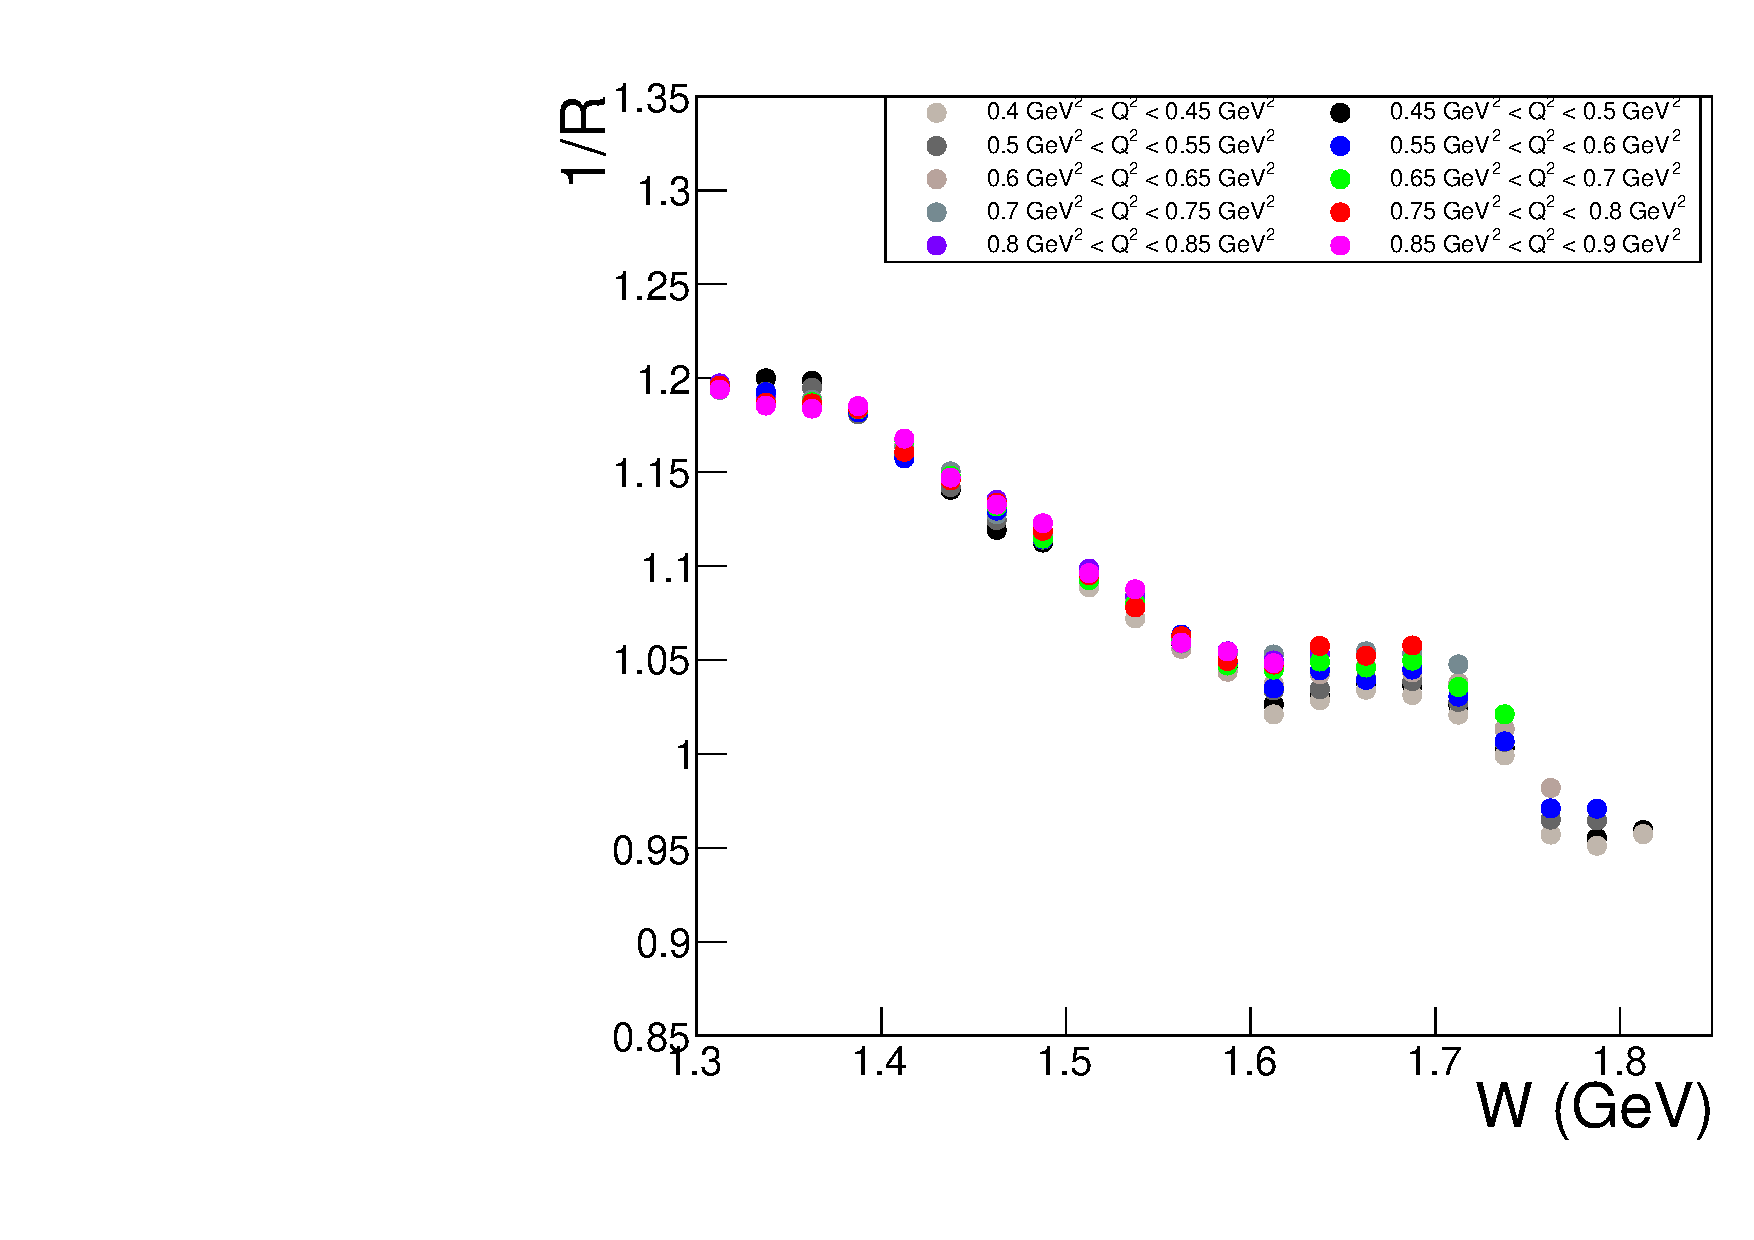
\includegraphics[width=8cm]{pictures/rad_corr/rad_corr_all_q2.pdf}
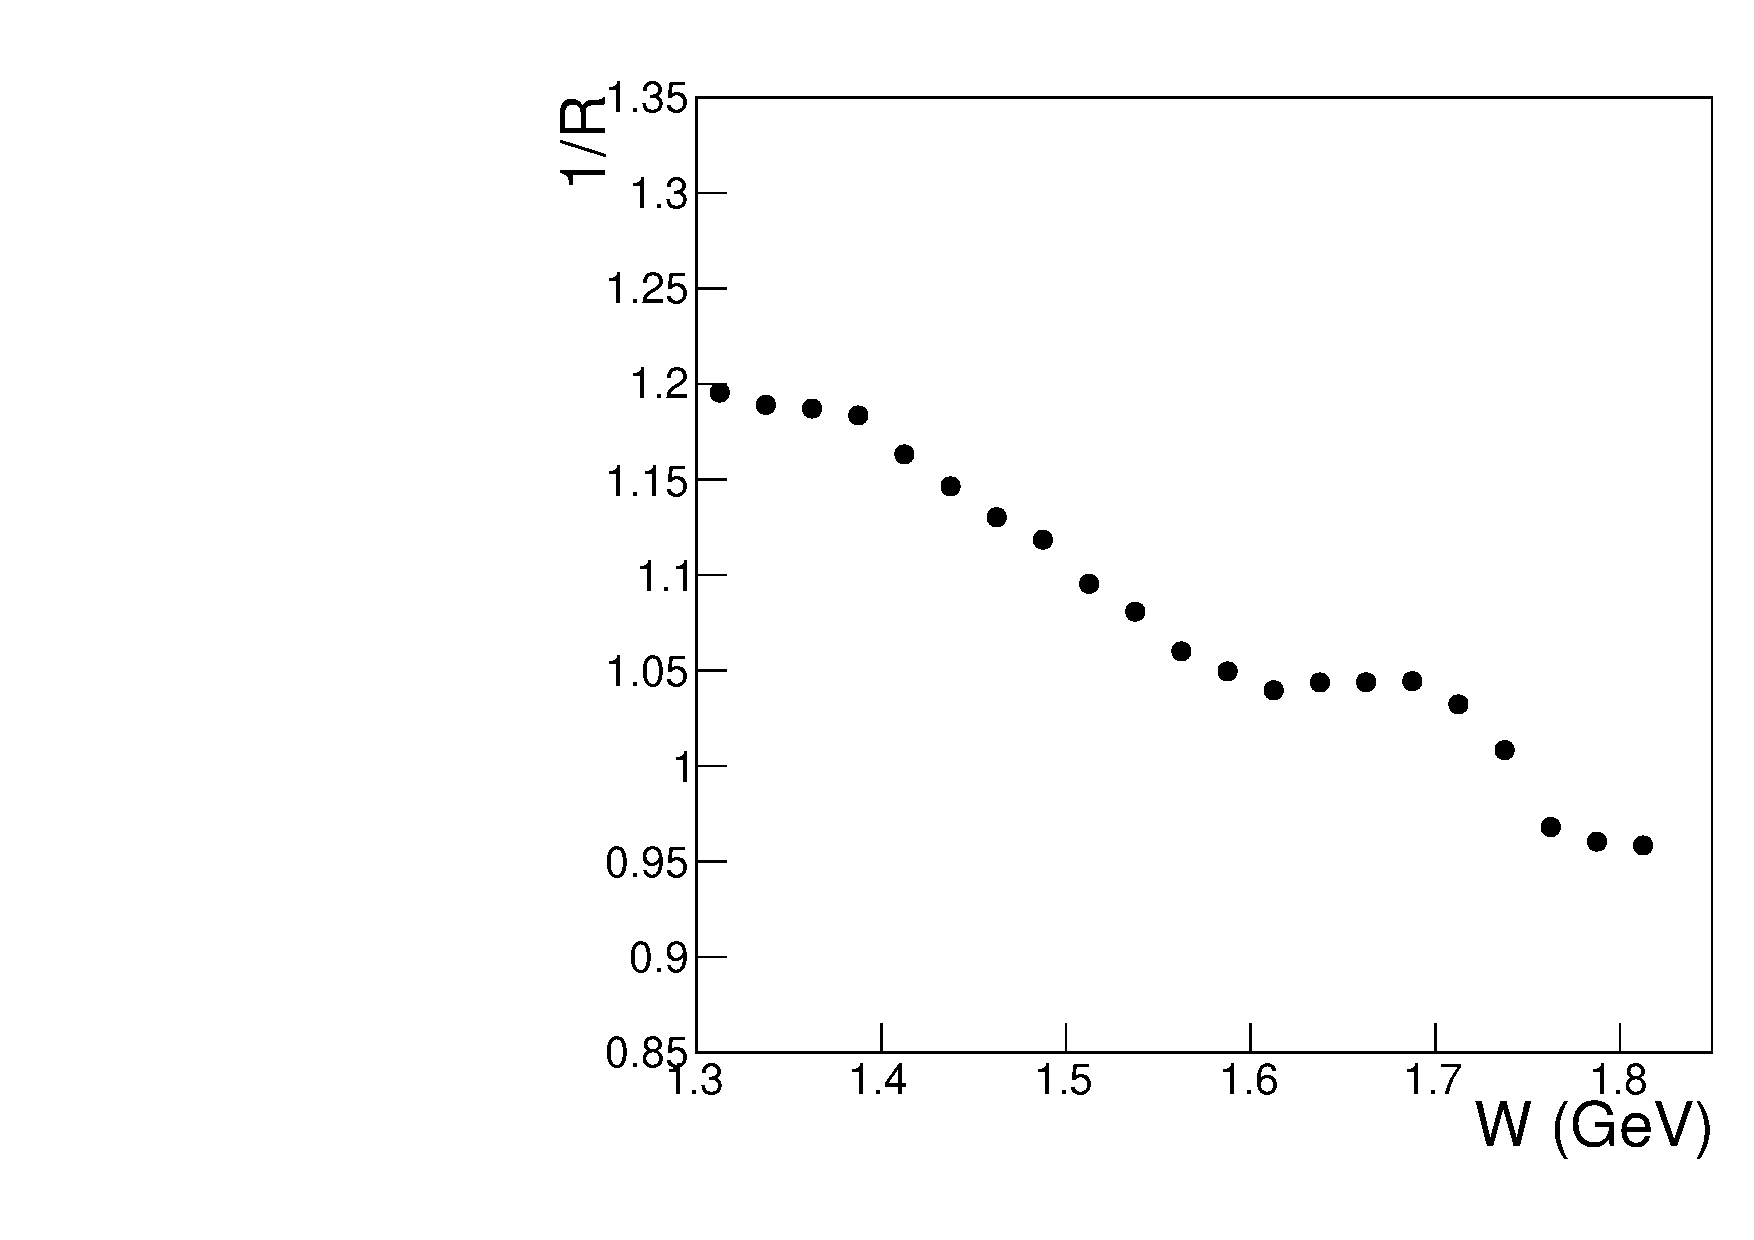
\includegraphics[width=8cm]{pictures/rad_corr/rad_corr_avrg.pdf}
\caption{\small One over radiative correction factor (see formula~\ref{expcrossect})
as function of $W$, for various bins over $Q^{2}$ (left plot) and averaged over all  $Q^{2}$ bins (right plot).} \label{radcorrfact}
\end{center}
\end{figure}

It should be noted that to account for radiative effects, the new double-pion event generator uses the well
known approach taken from Mo and Tsai~\cite{Mo:1968cg}.
In this approach the soft part is evaluated
explicitly, while for the calculation of the hard part the "inclusive" hadronic
tensor is used. The applicability
of this approximation for the hard part of
radiative effects is subject of special
attention. The single-differential double-pion cross sections~(\ref{inegr5diff}) obtained in this analysis represent the over four
variables integrated five-differential cross sections. This
integration considerably reduces the influence of
the final hadron kinematics on
the radiative correction factor. Therefore,
the "inclusive" Mo and Tsai procedure is in the case of double-pion cross sections more
applicable than in a case
of non-integrated cross sections that are typically obtained for instance in the single-pion data analysis.

It also should be mentioned that this correction should be applied before the empty cells (see Sect.~\ref{zero_acc}) are filled, since the cross sections that are used for the purpose of filling empty cells are already corrected for radiative effects.


\section{Efficiency evaluation}
\label{eff_aval} 

For the efficiency calculation the Monte Carlo event generator of
the Genova group is used. This event generator uses the JM05 model~\cite{JM05} for double-pion channel. Although the cross sections on which the event generator is based do not include the latest modifications of the JM model~\cite{Mokeev:2008iw,Mokeev:2012vsa,Mokeev:2015lda}, it describes the data well enough to use it for the purpose of the efficiency evaluation. 

To take into account the multi-pion background, three-pion events are generated simultaniously with the double-pion ones, the relative weight of these two channels is determined according to their integral cross sections at the photon point, see Fig.~\ref{fig:eff_2pi_3pi}. The event generator does not assume any model for the channel $e p \rightarrow e'p'\pi^{+}\pi^{-}\pi^{0}$, so for this channel phase space distributions are generated. It needs to be mentioned that even at high $W$ (around 1.8 GeV) three-pion background contributes only few percent to the double-pion events that survive after the exclusivity cut (see Sect.~\ref{excl_cut}). 

\begin{figure}[htp]
\begin{center}
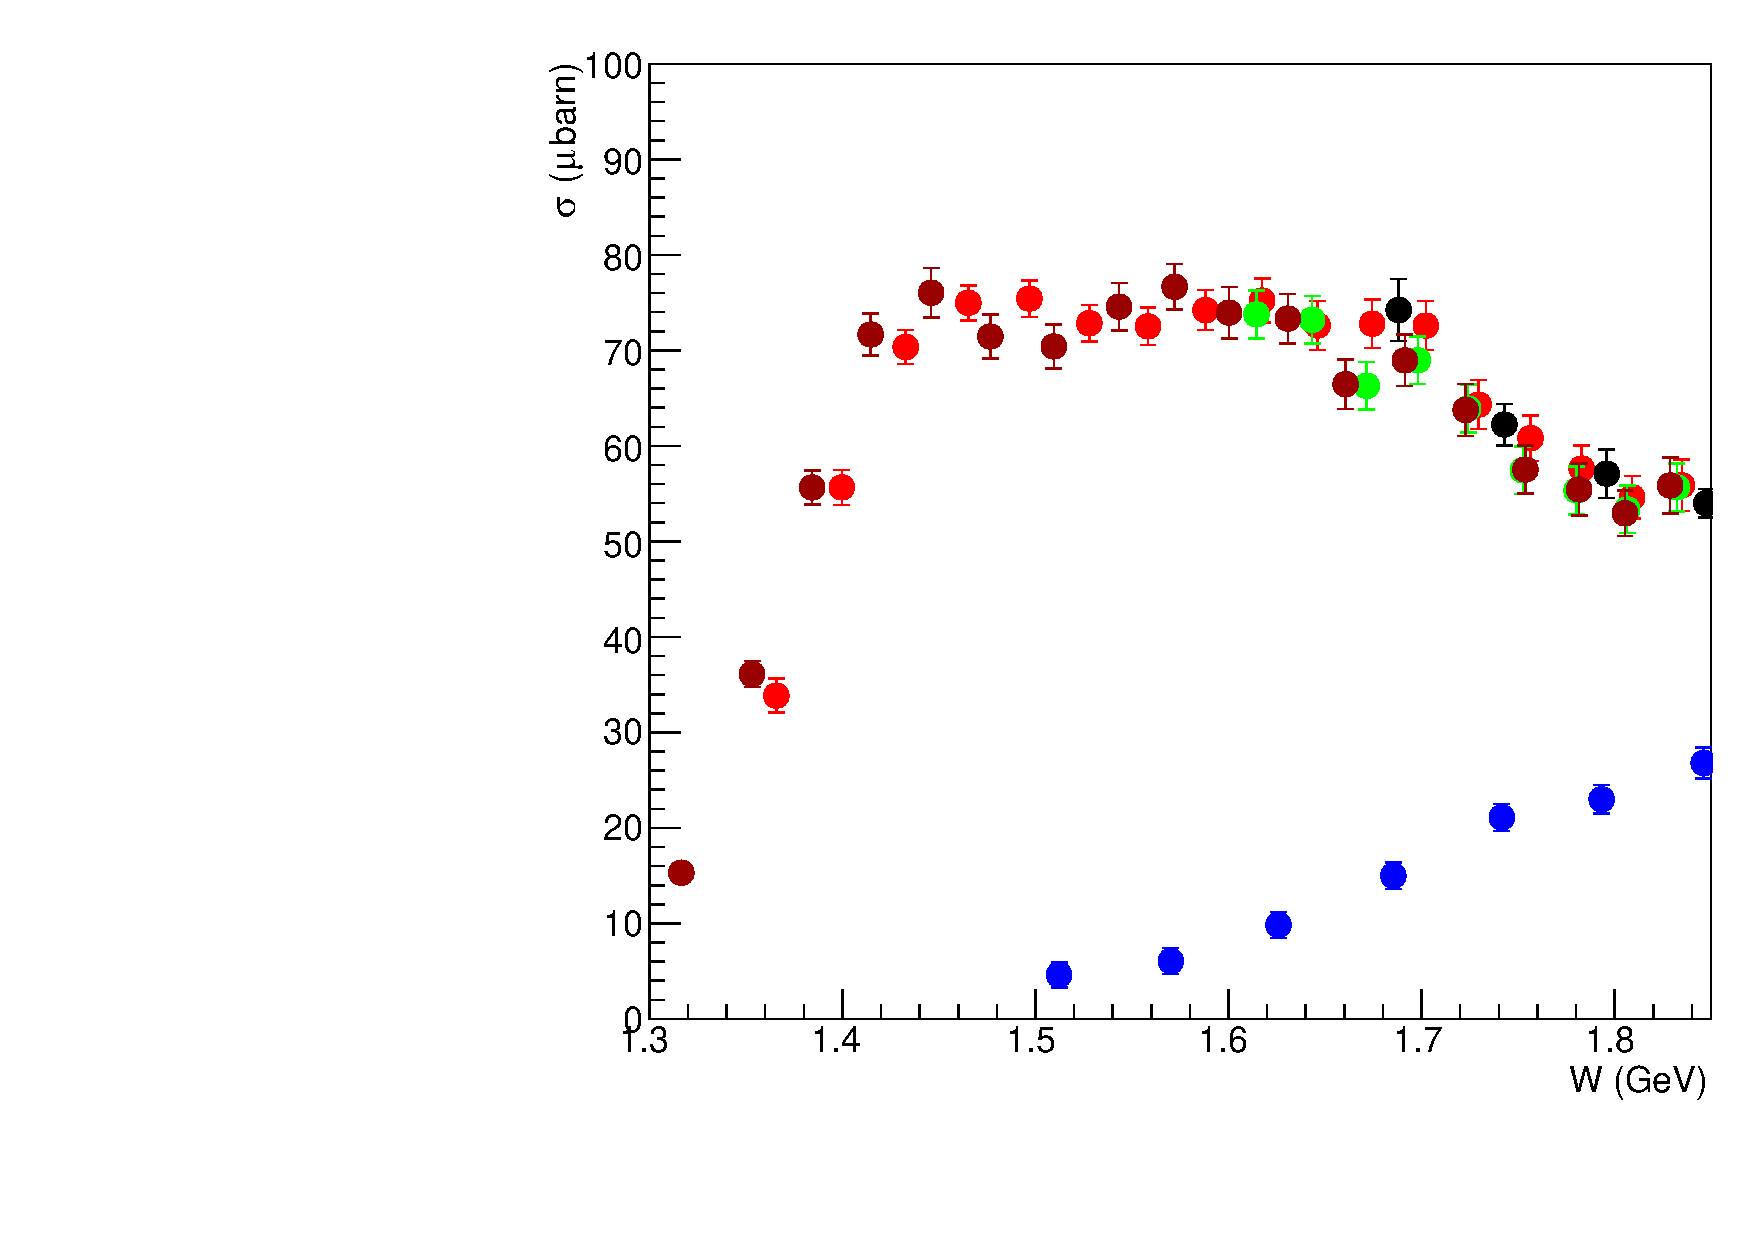
\includegraphics[width=8cm]{pictures/cross_sction/efficiency/2pi_3pi.pdf}
\caption{\small Integral cross sections of the reactions $e p \rightarrow e'p'\pi^{+}\pi^{-}$ and $e p \rightarrow e'p'\pi^{+}\pi^{-}\pi^{0}$ at the photon point. Black and red circles are double-pion data from~\cite{Wu:2005wf}. Green and brown circles are double-pion data from~\cite{ABBHHM:1968aa}. Blue cicrcles are three-pion data from~\cite{Erbe:1970cq}.} \label{fig:eff_2pi_3pi}
\end{center}
\end{figure}

All generated events are passed through GSIM, GPP and RECSIS. The parameters for the simulation are taken to be the same as in~\cite{Markov:phd}. After applying all cuts and corrections described above, the reconstructed events are compared with the data. As it is seen on the left side of Fig.~\ref{fig:eff_data_sim} MC reconstructed events reproduce the data rather well.

On the right side of Fig.~\ref{fig:eff_data_sim} the average efficiency in five-dimensional kinematical cell is shown as functions of the hadron variables that describe the double-pion final state. No distributions show any significant efficiency variation. 

The efficiency in some five-dimensional cells is not determined precisely enough, this leads to the fact that the cross sections obtained in them are not reliable. These cells should be 
 excluded from the analysis and treated as empty cells (see Sect.~\ref{zero_acc}).
In order to determine the criterion for cell exclusion the distribution shown in Fig.~\ref{fig:eff_err} is produced.
This figure shows the relative efficiency error (absolute efficiency error is given by~\ref{efferror}) that is plotted versus efficiency, color code in this figure represents the number of five-dimensional cells. As it is seen in  Fig.~\ref{fig:eff_err} cells with relative efficiency errors greater than 30\% are clustered along horizontal stripes. This effect  can be explained taking into account that efficiency is obtained by division of two integer numbers, and it indicates too small statistics of generated events that in turn leads to higher efficiency errors. Moreover these horizontal stripes contain many cells with extremely small efficiency values that one can not count on anyway. Therefore,  the five-dimensional cells that are located above the horizontal red line in Fig.~\ref{fig:eff_err} are excluded from the analysis and treated as empty cells (see Sect.~\ref{zero_acc}).

 
\begin{figure}[htp]
\begin{center}
\frame{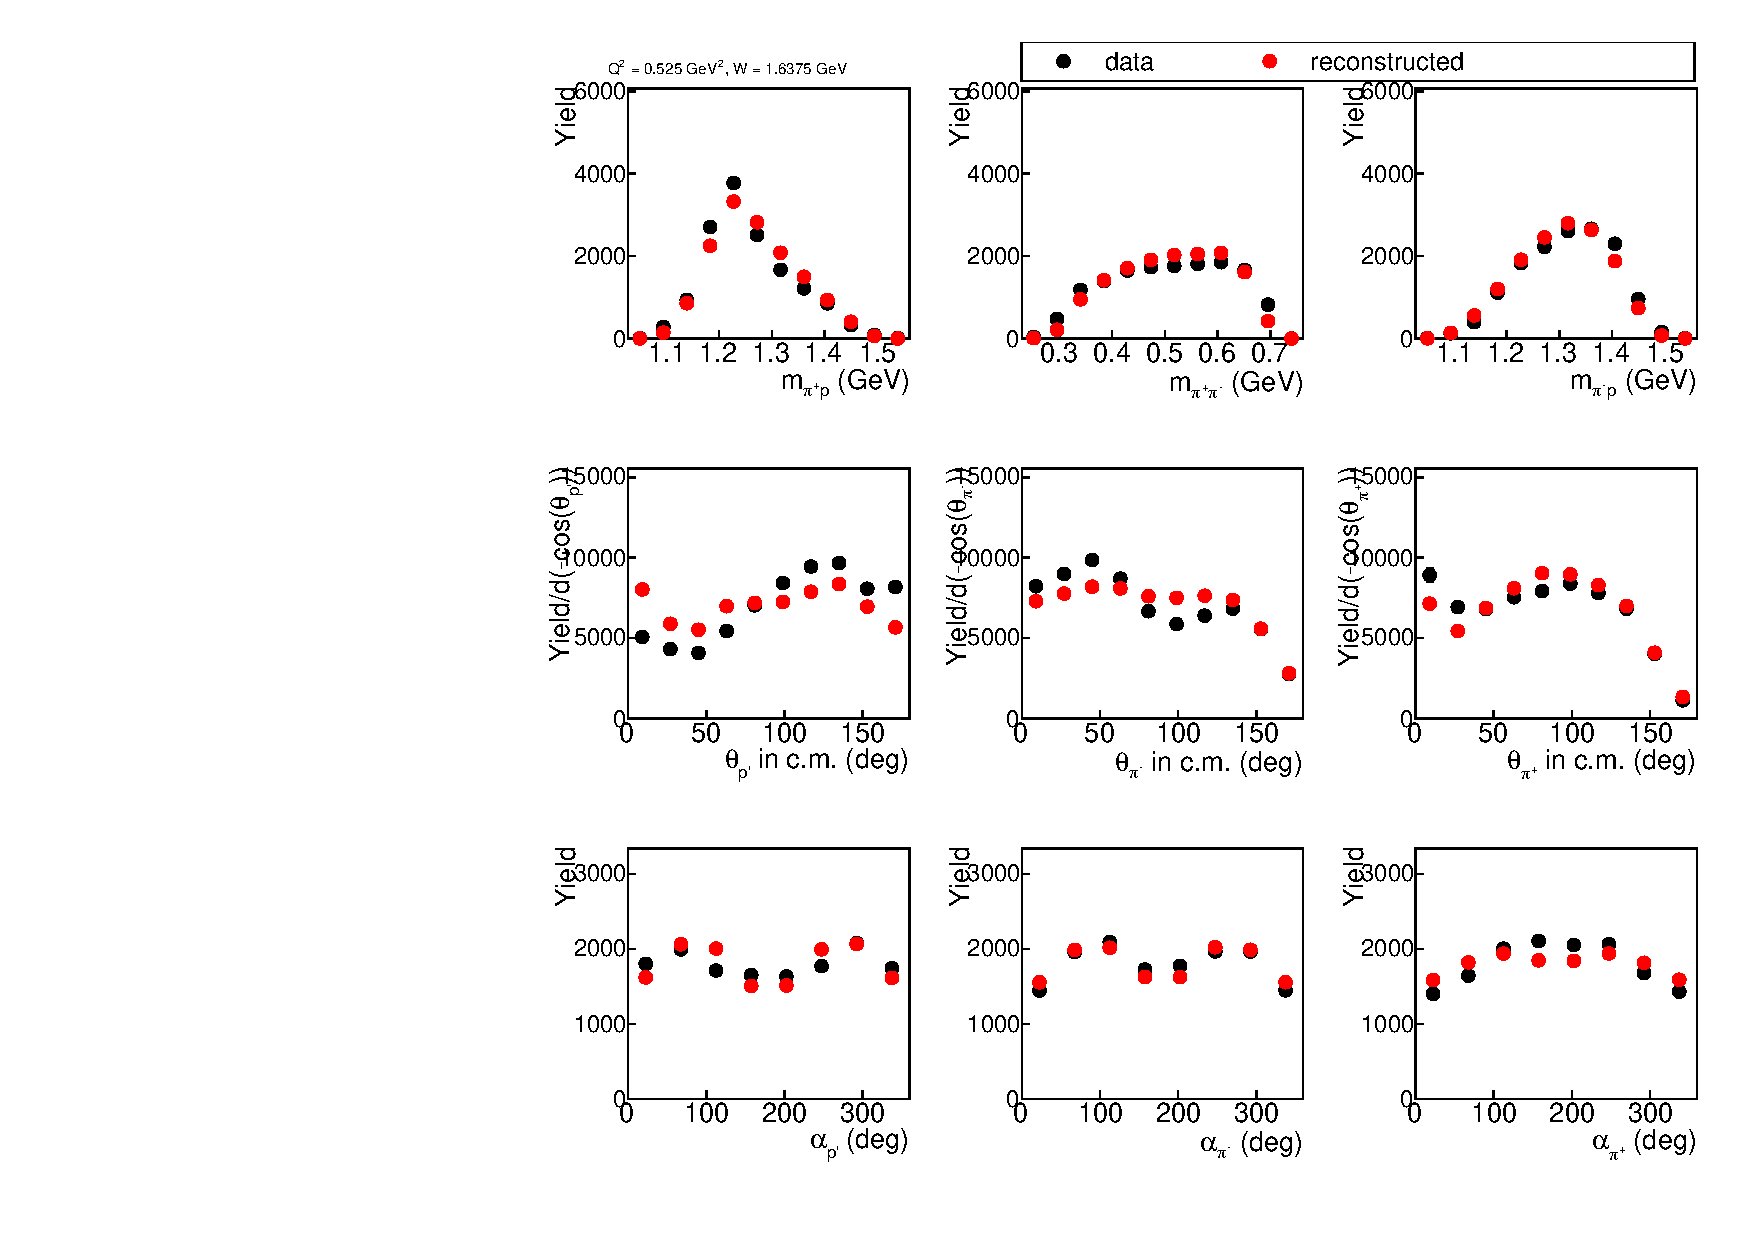
\includegraphics[width=8cm]{pictures/cross_sction/efficiency/data_rec_plot.pdf}}
\frame{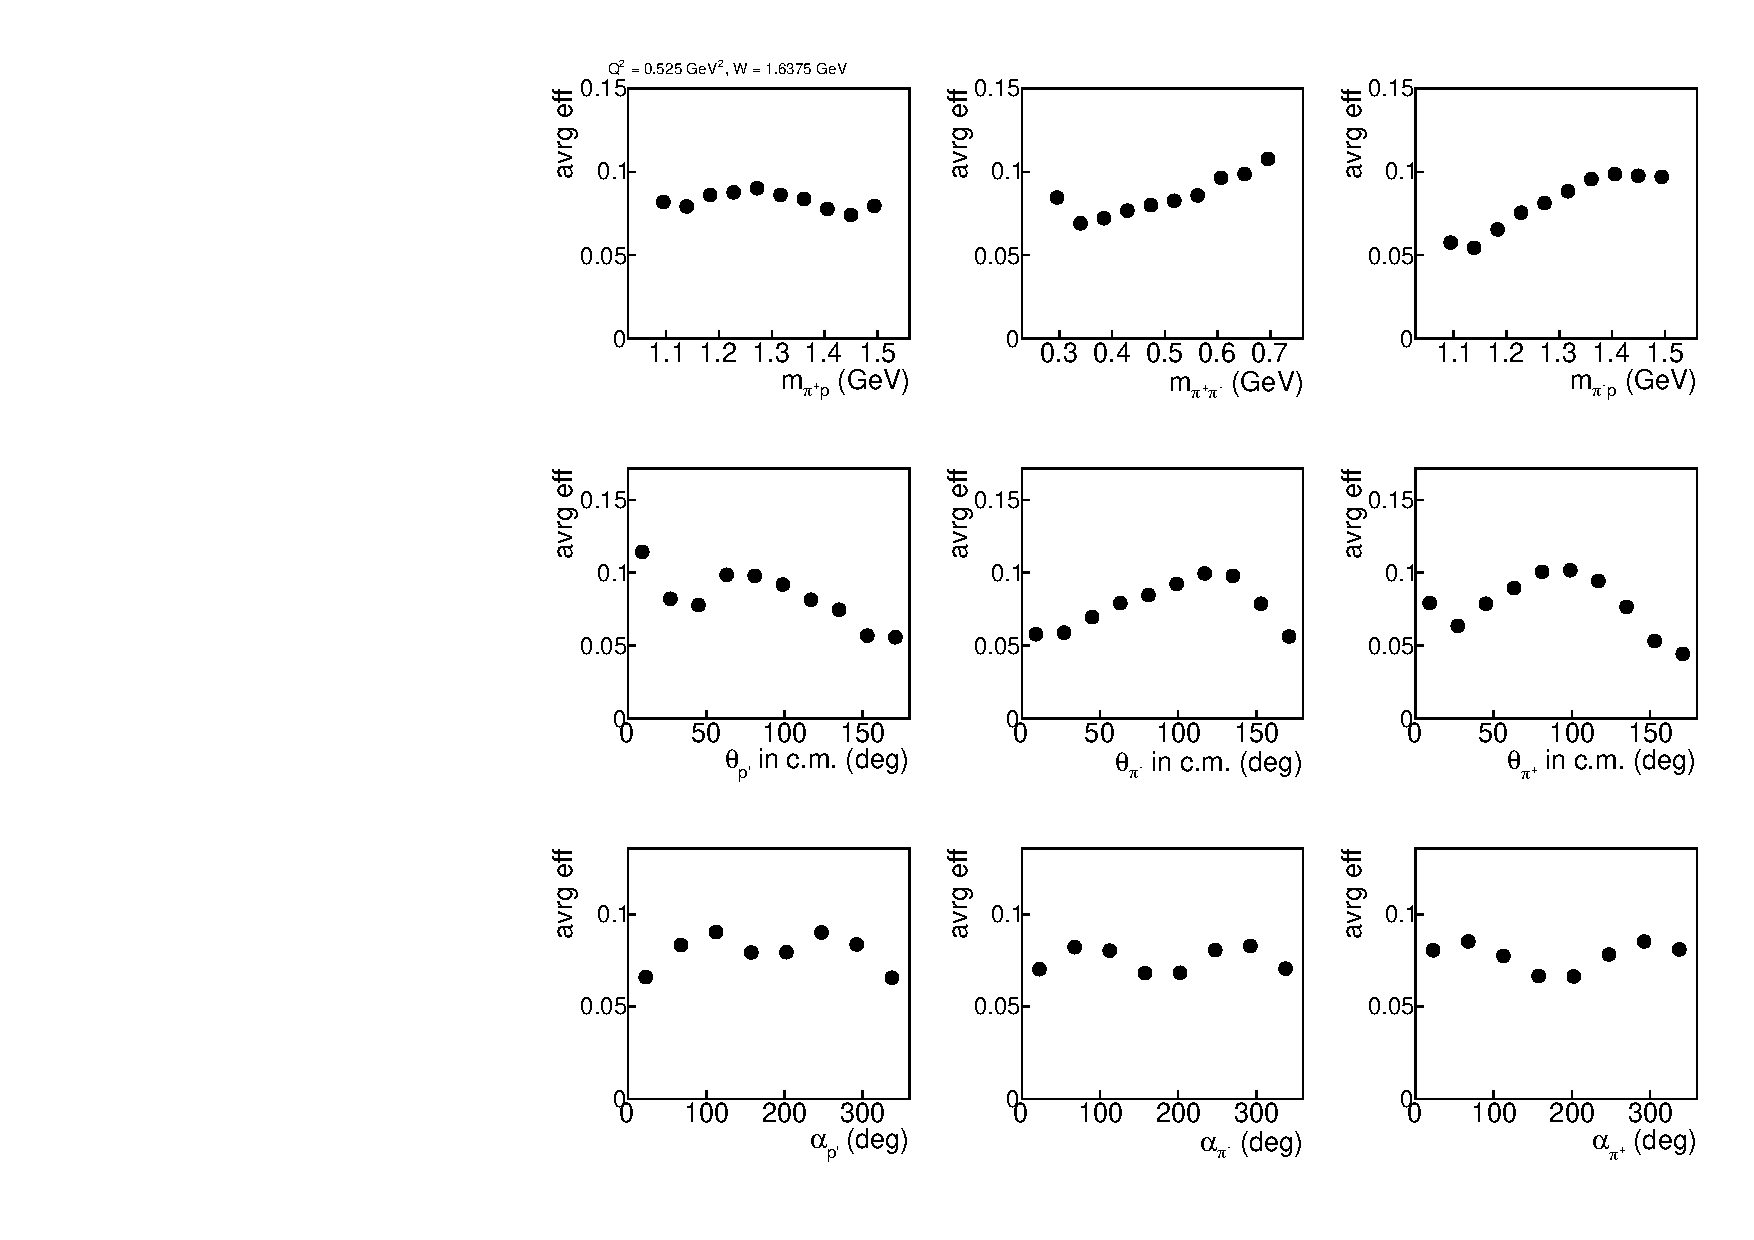
\includegraphics[width=8cm]{pictures/cross_sction/efficiency/eff_plot.pdf}}
\caption{\small Plots in the left frame show the comparison of data and reconstructed MC yields as functions of various hadronic variables that describe the double-pion final state. Plots in the right frame show the average efficiency in the five-dimensional kinematical cell as functions of the final state hadronic variables. All distributions are given for one particular bin in $W$ and $Q^2$ ($W = 1.6375$~GeV, $Q^2 = 0.525$~GeV$^2$).} \label{fig:eff_data_sim}
\end{center}
\end{figure}


\begin{figure}[htp]
\begin{center}
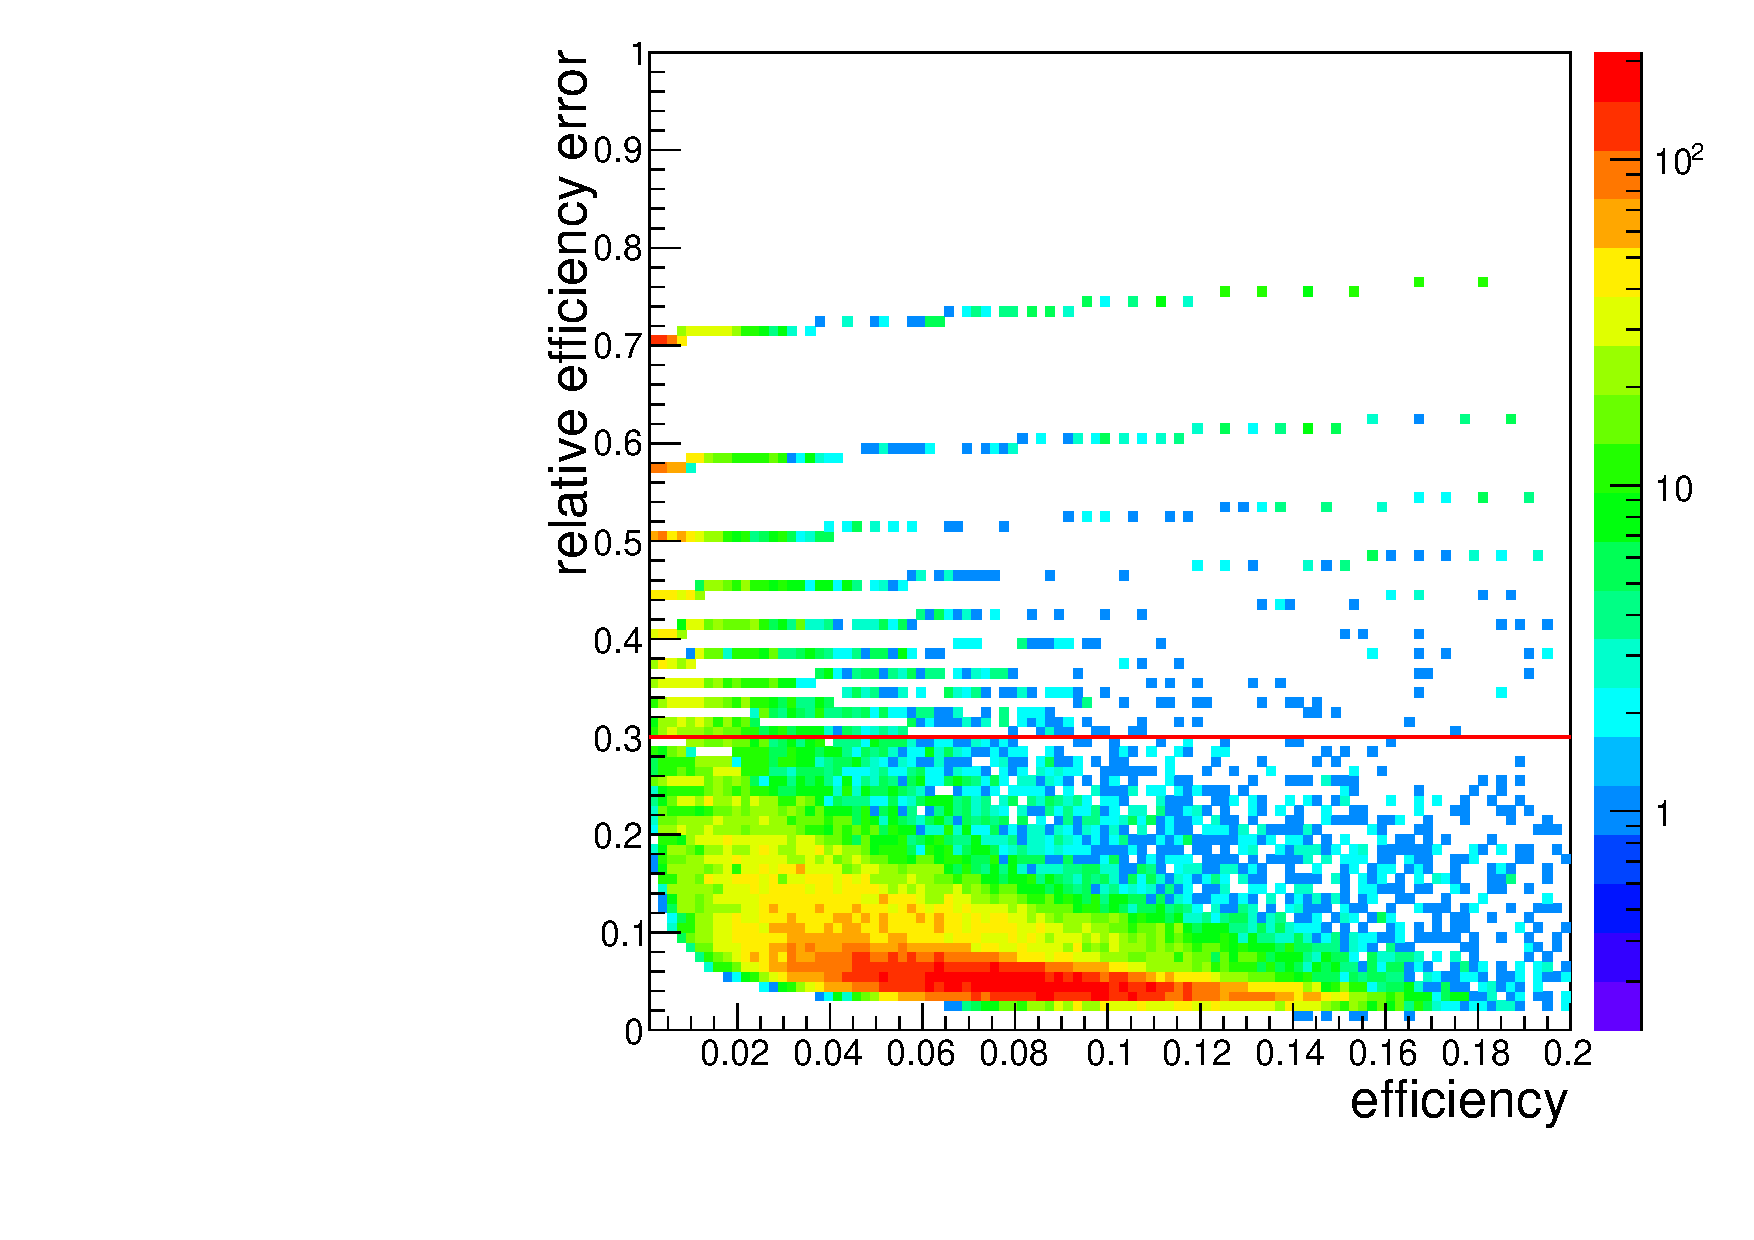
\includegraphics[width=7cm]{pictures/cross_sction/efficiency/eff_err.pdf}
\caption{\small Relative efficiency error versus efficiency for one particular bin in $W$ and $Q^2$ ($W = 1.6375$~GeV, $Q^2 = 0.525$~GeV$^2$). Color code shows the number of five-dimensional cells.} \label{fig:eff_err}
\end{center}
\end{figure}


\section{Filling kinematical cells with zero acceptance}
\label{zero_acc} 

\begin{figure}[htp]
\begin{center}
\frame{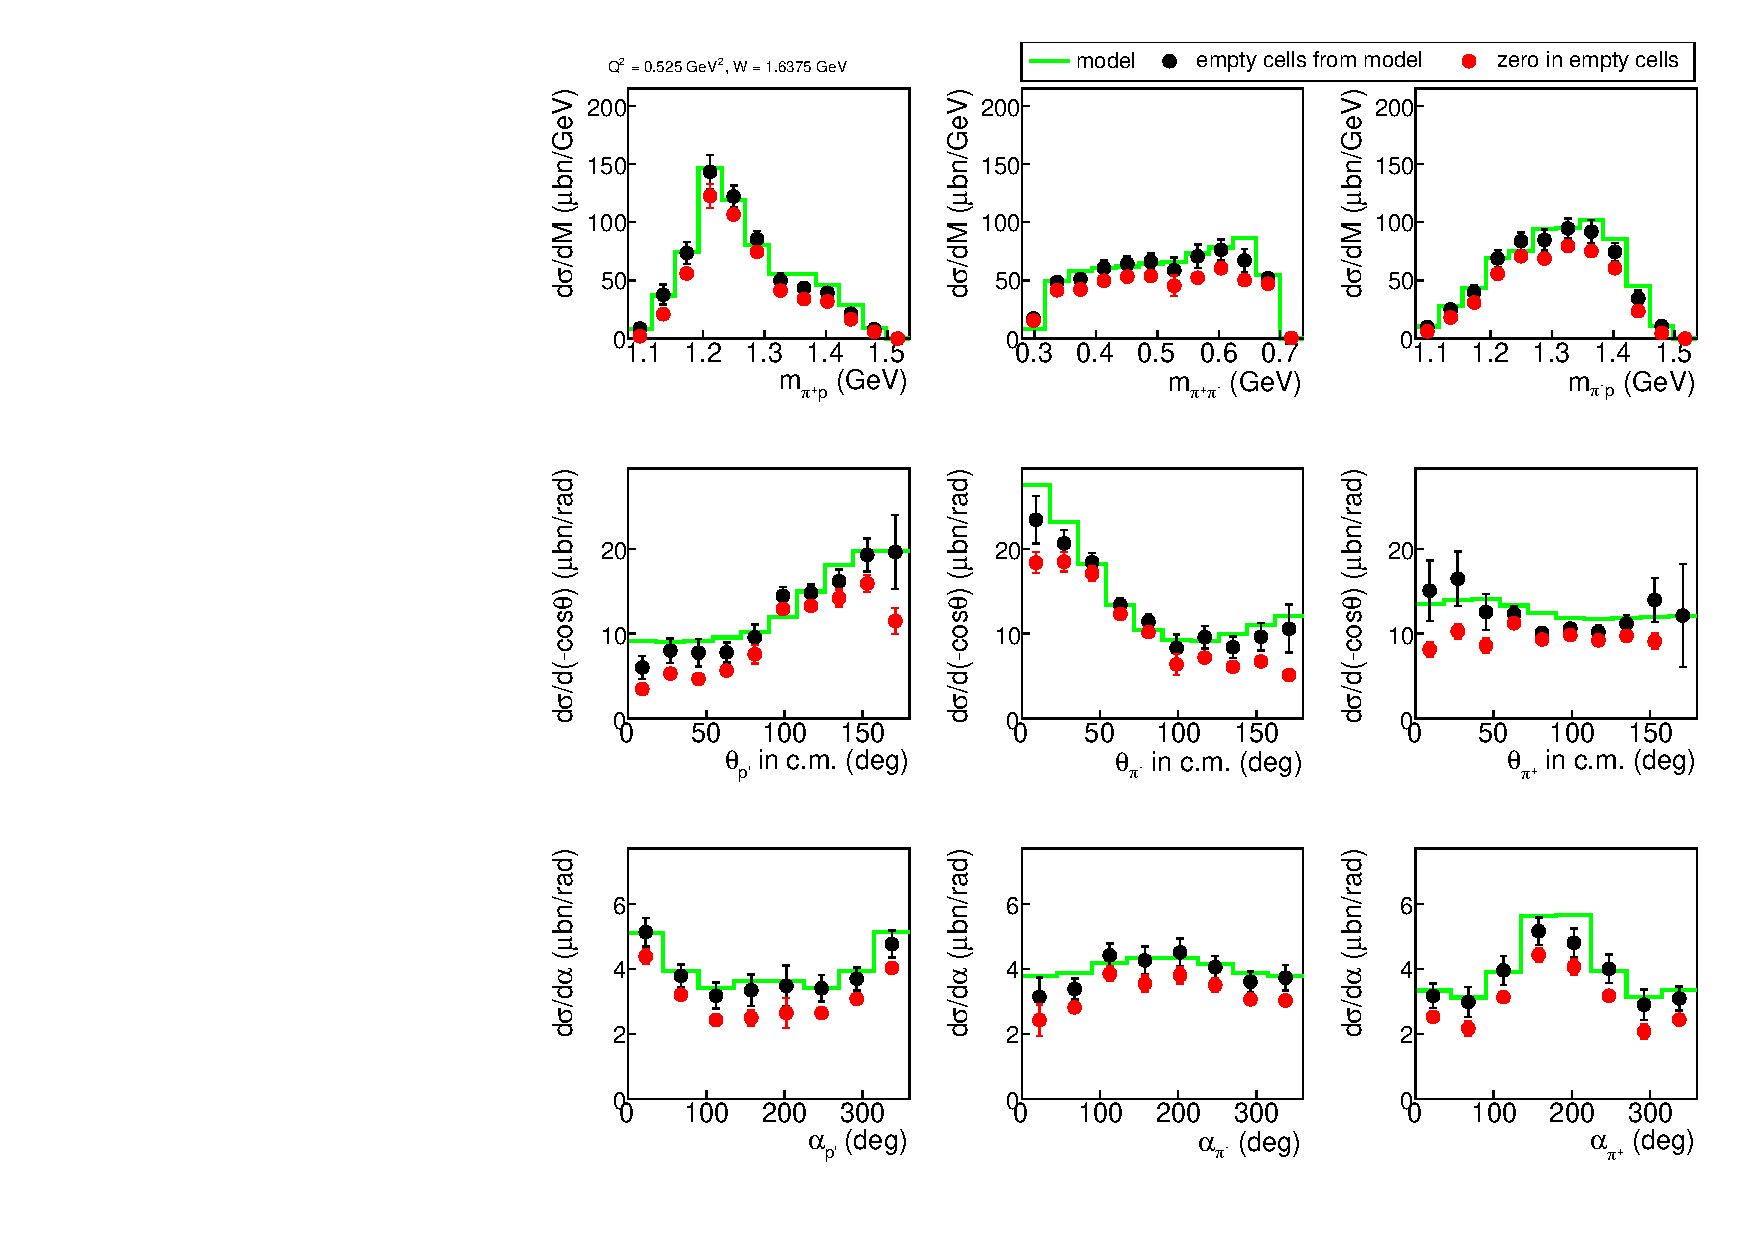
\includegraphics[width=8cm]{pictures/cross_sction/topologies/cr_sec_pim.pdf}} \\
\frame{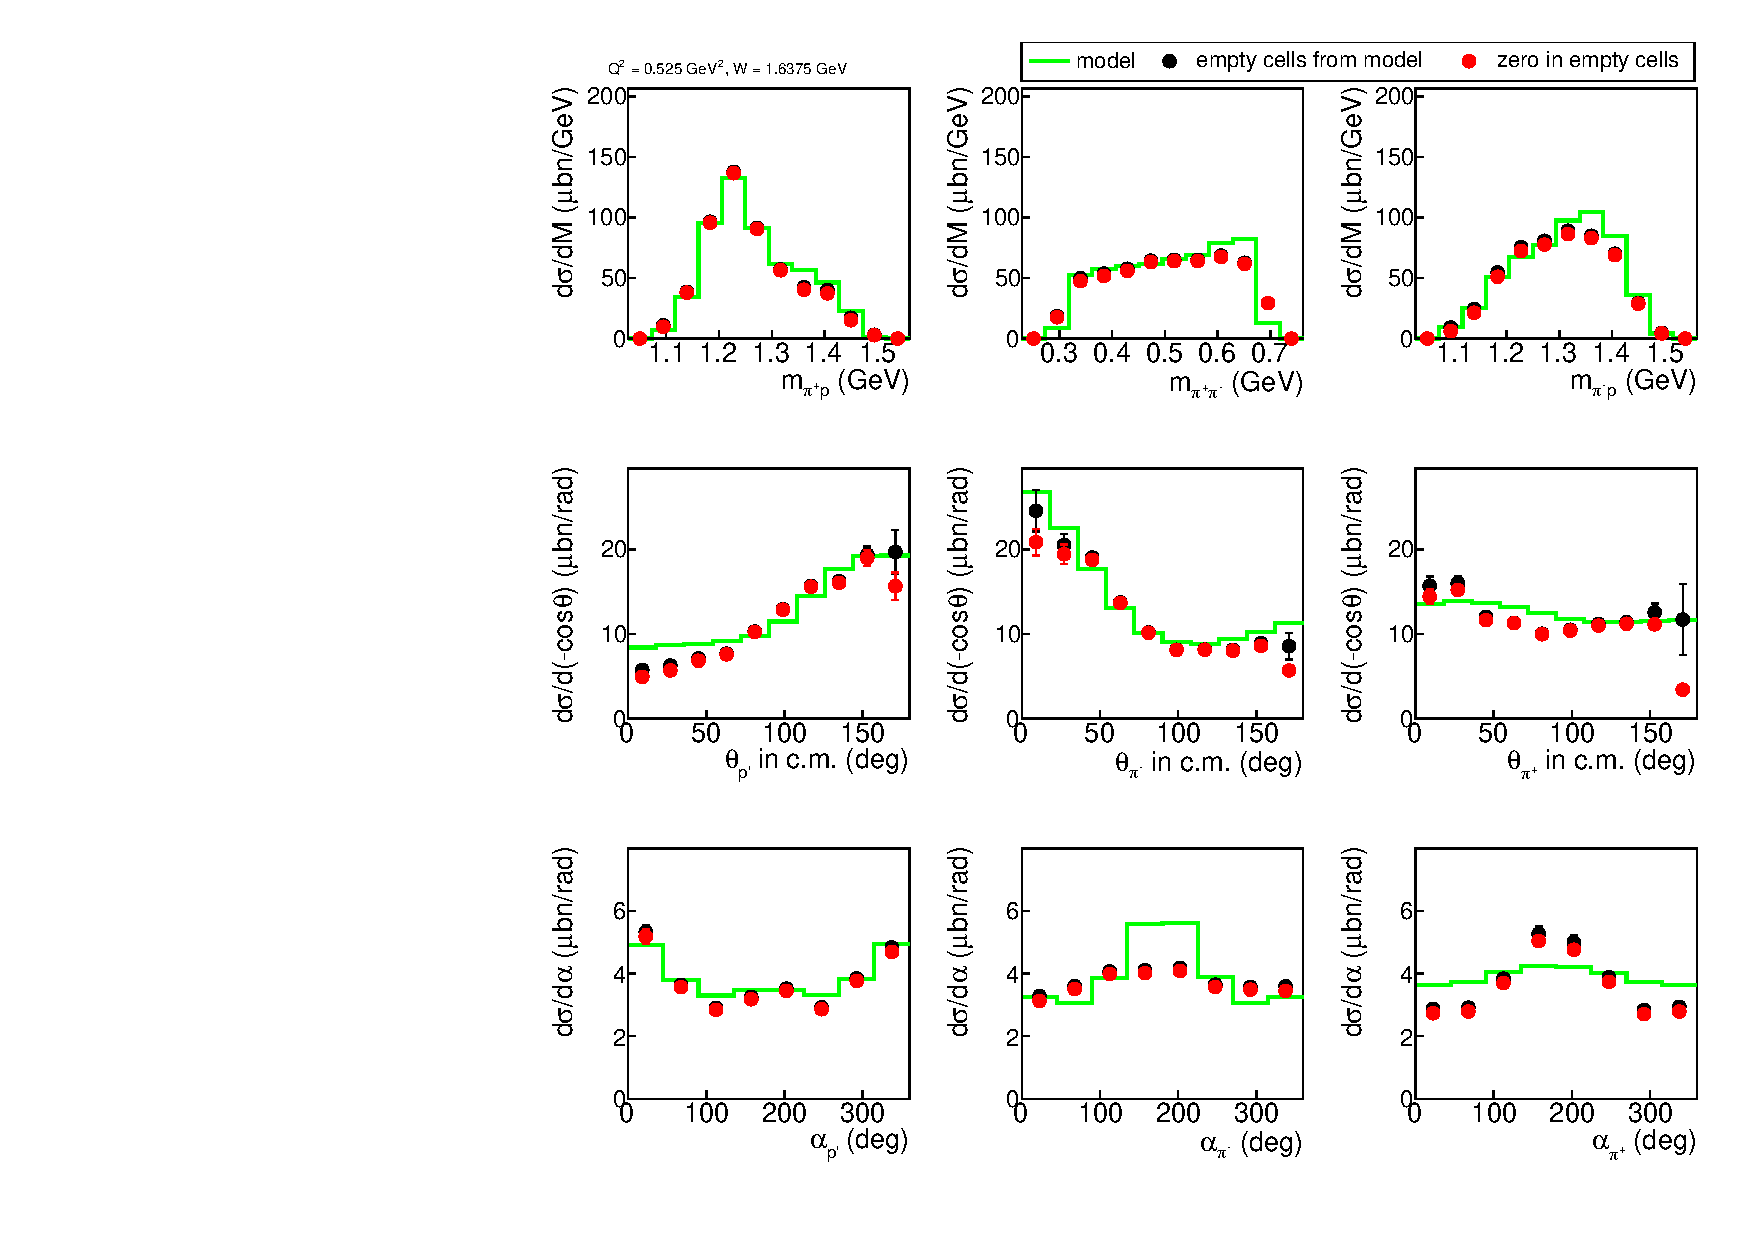
\includegraphics[width=8cm]{pictures/cross_sction/topologies/cr_sec_all_top.pdf}}
\frame{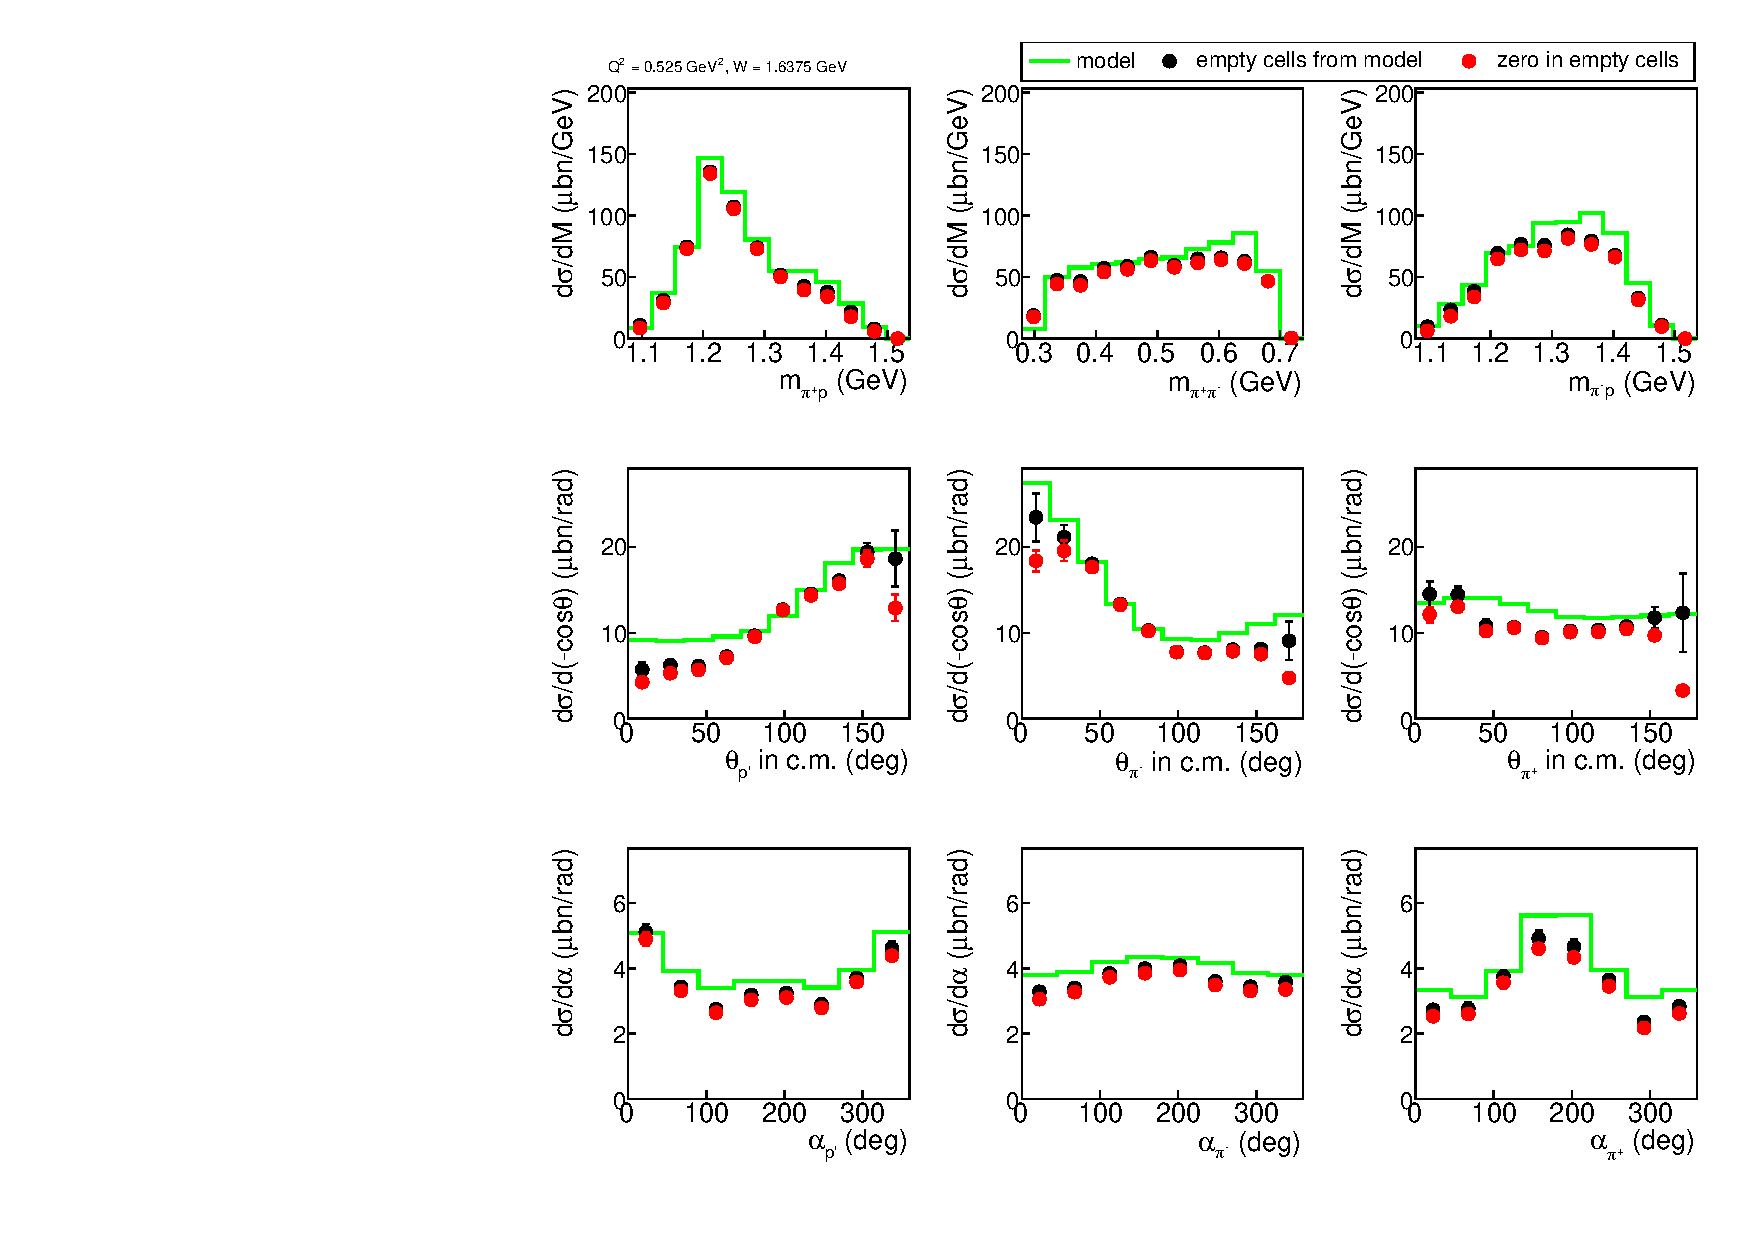
\includegraphics[width=8cm]{pictures/cross_sction/topologies/cr_sec_max_eff.pdf}}
\caption{\small Comparison of various ways of combining topologies. Plots in the top frame are for the case when the cross sections are  obtained using the topology where $\pi^{-}$ is missing combined with the exclusive topology. Plots in the bottom left frame are for the case when the cross sections are obtained using the sum of data and reconstructed events for all four topologies. Plots in the bottom right frame are for the case when the cross sections are obtained using the selection of five-dimensional cells based on the maximum efficiency. See text for more details. In all plots the red circles are for the cross sections with unfilled empty cells and the black circles are for the cross sections with filled empty cells. Green curves show the cross sections that are used for the purpose of filling empty cells. All distributions are given for one particular bin in $W$ and $Q^2$ ($W = 1.6375$~GeV, $Q^2 = 0.525$~GeV$^2$).} \label{fig:topologies}
\end{center}
\end{figure}

Since the CLAS detector does not cover full $4\pi$ solid angle, there are some blind areas or so-called "empty cells" in the kinematic phase space of the double-pion production. 
In the case when fully differentional cross sections are obtained (for example in single pion production analyses) the presence of these cells is not a problem of big importance. 
Due to the statistical limitations in the double-pion analyses only the single-differential cross sections can be obtained. It means that the five-differential cross sections need to be integrated over four variables~(see formulae~\ref{inegr5diff}). To obtain correct integrals, some assumptions on the cross sections in the empty cells are needed. It makes the problem of filling  empty cells a point of special attention.


The map of the empty cells is determined by the Monte Carlo simulation. A cell is treated as empty, if it contains generated events, but does not contain any reconstructed events. One should not confuse these cells with those that contain both generated and reconstructed events, but do not contain data. The latter do not contain real events due to the limited experiment duration, and should not be filled since normalization on the charge in Faraday cup is applied.

To consider contributions from empty cells to the integrals~(\ref{inegr5diff})  in detail model assumptions on the cross sections in these cells are needed. Recently for the purpose of the development of new double-pion event generator~\cite{Skorodum:EG} a special procedure that allows to obtain the five-differential double-pion cross sections in the given kinematical cell was worked out. This procedure employs the five-differential cross sections from the recent version of the JM15 model fit to all results on charged double pion photo- and electroproduction cross sections from  CLAS (both published and preliminary~\cite{Ripani:2002ss,Mokeev:2012vsa,Fedotov:2008aa,Golovach:note}). 
In the area not yet covered by CLAS data an additional extrapolation technique was applied, that included additional world data on $W$ dependencies of double-pion photoproduction integrated cross sections~\cite{Wu:2005wf,ABBHHM:1968aa}.
The set of the cross sections obtained using this procedure was used for the purpose of filling empty cells in this analysis.





 In Fig.~\ref{fig:topologies} the single-differential cross sections are plotted for the two cases: when empty cells are not filled (red circles) and when empty cells are filled by the way described above (black circles). The cross sections that are used to fill empty cells are shown by the green curves. The plot in the top frame of Fig.~\ref{fig:topologies}  corresponds to the topology where $\pi^{-}$ is missing combined with the exclisive topology, while the two plots in the bottom frames correspond to different ways of combining of all avaliable topologies (ways in which the topologies may be combined are  described in more detail in Sect.~\ref{var_top}). 
 
The plot in the left bottom frame in Fig.~\ref{fig:topologies} corresponds to the method of the topologies combination that is selected to be the best. As it can be seen in the left bottom frame in Fig.~\ref{fig:topologies} the contribution from empty cells to the total cross sections is reasonably small. Although the cross sections that are used to fill empty cells describe the data well an additional 50\% relative error is assigned to the part of the cross section that comes from the empty cell contributions. For finally obtained cross sections (shown by black circles) this additional error is combined with the total statistical one.




\section{Combination of various topologies}
\label{var_top}

It is mentioned in Sect.~\ref{excl_cut} that the topology where $\pi^{-}$ is missing combined with the exclusive one accounts about 80\% of all double-pion events. In previously published analyses~\cite{Fedotov:2008aa,Isupov:note} only these two topologies were used to obtain final cross sections.

In this analysis it is found that the use of only the combination of the exclusive and  $\pi^{-}$ missing topologies leads to significant contributions from empty cells to the total cross sections in some phasespace regions (see plot in the top frame of Fig.~\ref{fig:topologies}). Moreover, the last point in $\theta_{\pi^{+}}$  angular distribution does not contain data at all and the cross section in this point is totally determined by the procedure of filling empty cells as described in Sect.~\ref{zero_acc}.

Hence to minimize the part of the cross section that comes from filling of the empty cells and therefore the model dependence of the obtained cross sections, it was decided to use all avaliable topologies.

There are two methods in which topologies can be combined. One of them is chosen as preferable and used to obtain the final cross sections. In this method data events for all topologies are summed up in each five-dimensional kinematical cell. The same is done for the reconstructed events, while the number of generated events remains the same. Then the cross sections are calculated in a usual way. The cross sections for the case when all topologies are combined by this method are shown in the bottom left frame of Fig.~\ref{fig:topologies}. One can see that the usage of this method allows to minimize the part of the cross section that comes from the empty cells contributions in comparison with the case when only the exclusive and $\pi^{-}$ missing topologies are used. Moreover even the last point in $\theta_{\pi^{+}}$  angular distribution now is partially determined by data and therefore less model dependent.

Another way to combine topologies is used to check the consistency of the results. In this way in each five-dimensional kinematical cell reconstructed and data events are taken from the topology that has maximum efficiency, while the number of generated events remains the same. The cross sections that are obtained using this method are shown in the bottom right frame of Fig.~\ref{fig:topologies}.  
Although this method gives almost the same result as the previous one, it has several shortcomings. One of them is slightly bigger contribution from empty cells. Another one is the fact that this method does not allow to use the whole avaliable statistics of the data. As a result the error of the obtained cross sections becomes a little bit higher than in the previous method. That is why this method is not chosen as a primary one.
The difference between the cross sesctions obtained by the two methods described above is used as part of the systematical error of the integrated cross sections (see Sect.~\ref{var_top_err}).


Finally it needs to be mentioned that independently of the way the cross sections are calculated (see all plots in Fig.~\ref{fig:topologies}), the final cross sections obtained after filling the empty cells are very close to each other. That indicates the stability and reliability of the cross section extraction procedure.




